%%%%%%%%%%%%%%%%%%%%%%%%%%%%%%%%%%%%%%%%%%%%%%%
%%%     Declarations (skip to Begin Document, line 88, for parts you fill in)
%%%%%%%%%%%%%%%%%%%%%%%%%%%%%%%%%%%%%%%%%%%%%%%

%%\documentclass[10pt]{article}
%%\documentclass[10pt]{report}
\documentclass[letterpaper]{article}
\usepackage{geometry}
%\usepackage{xcolor}
\usepackage[table]{xcolor}
\usepackage{amsmath}
\usepackage[some]{background}
%\usepackage{lipsum}
%\usepackage{natbib}

% C I T A T I O N S
\usepackage[backend=biber, style=apa]{biblatex}  
%\usepackage{biblatex} 
\addbibresource{paperpile.bib}

\usepackage[hidelinks]{hyperref}

% C A P T I O N S
%\usepackage{caption, copyrightbox}
%\captionsetup{justification=centering, labelfont=sc, labelsep=endash}

% Tables
\usepackage{float}
\usepackage[utf8]{inputenc}
\usepackage{tabularx}
\usepackage{booktabs}
\usepackage{longtable}

\usepackage{diagbox} %table split headers
\usepackage{longtable}
\usepackage{array}
\usepackage{rotating}
\usepackage{eqparbox}
\usepackage{makecell, caption, booktabs}

% Stuff needed to get table to span pages
\usepackage{enumitem}
%\usepackage{array, booktabs, longtable}
\newcolumntype{x}[1]{>{\raggedright}p{#1}}

\usepackage{etoolbox}
\AtBeginEnvironment{longtable}{%
    \setlist[itemize]{nosep,     % <-- new list setup
                      topsep     = 0pt       ,
                      partopsep  = 0pt       ,
                      leftmargin = *         ,
                      label      = $\bullet$ ,
                      before     = \vspace{-\baselineskip},
                      after      = \vspace{-0.5\baselineskip}
                        }
                           }% end of AtBeginEnvironment
% End table span
% Listings
\usepackage{listings}

\usepackage{geometry}  % Lots of layout options.  See http://en.wikibooks.org/wiki/LaTeX/Page_Layout
\geometry{letterpaper}  % ... or a4paper or a5paper or ... 
\usepackage{fullpage}  % somewhat standardized smaller margins (around an inch)
\usepackage{setspace}  % control line spacing in latex documents
\usepackage[parfill]{parskip}  % Activate to begin paragraphs with an empty line rather than an indent

\usepackage{amsmath,amssymb}  % latex math
\usepackage{empheq} % http://www.ctan.org/pkg/empheq
\usepackage{bm,upgreek}  % allows you to write bold greek letters (upper & lower case)

% for typsetting algorithm pseudocode see http://en.wikibooks.org/wiki/LaTeX/Algorithms_and_Pseudocode
\usepackage{algorithmic,algorithm}  

\usepackage{graphicx}  % inclusion of graphics; see: http://en.wikibooks.org/wiki/LaTeX/Importing_Graphics
% allow easy inclusion of .tif, .png graphics
\DeclareGraphicsRule{.tif}{png}{.png}{`convert #1 `dirname #1`/`basename #1 .tif`.png}

% \usepackage{subfigure}  % allows subfigures in figure
\usepackage{caption}
\usepackage{subcaption}

\usepackage{xspace}
\newcommand{\latex}{\LaTeX\xspace}

\usepackage{color}  % http://en.wikibooks.org/wiki/LaTeX/Colors

\long\def\todo#1{{\color{red}{\bf TODO: #1}}}

\long\def\ans#1{{\color{blue}{\em #1}}}
\long\def\ansnem#1{{\color{blue}#1}}
\long\def\boldred#1{{\color{red}{\bf #1}}}
\long\def\boldred#1{\textcolor{red}{\bf #1}}
\long\def\boldblue#1{\textcolor{blue}{\bf #1}}

% Useful package for syntax highlighting of specific code (such as python) -- see below
\usepackage{listings}  % http://en.wikibooks.org/wiki/LaTeX/Packages/Listings
\usepackage{textcomp}


%%% The following lines set up using the listings package
\renewcommand{\lstlistlistingname}{Code Listings}
\renewcommand{\lstlistingname}{Code Listing}

%%% Specific for python listings
\definecolor{gray}{gray}{0.5}
\definecolor{green}{rgb}{0,0.5,0}

\lstnewenvironment{python}[1][]{
\lstset{
language=python,
basicstyle=\footnotesize,  % could also use this -- a little larger \ttfamily\small\setstretch{1},
stringstyle=\color{red},
showstringspaces=false,
alsoletter={1234567890},
otherkeywords={\ , \}, \{},
keywordstyle=\color{blue},
emph={access,and,break,class,continue,def,del,elif ,else,%
except,exec,finally,for,from,global,if,import,in,i s,%
lambda,not,or,pass,print,raise,return,try,while},
emphstyle=\color{black}\bfseries,
emph={[2]True, False, None, self},
emphstyle=[2]\color{green},
emph={[3]from, import, as},
emphstyle=[3]\color{blue},
upquote=true,
morecomment=[s]{"""}{"""},
commentstyle=\color{gray}\slshape,
emph={[4]1, 2, 3, 4, 5, 6, 7, 8, 9, 0},
emphstyle=[4]\color{blue},
literate=*{:}{{\textcolor{blue}:}}{1}%
{=}{{\textcolor{blue}=}}{1}%
{-}{{\textcolor{blue}-}}{1}%
{+}{{\textcolor{blue}+}}{1}%
{*}{{\textcolor{blue}*}}{1}%
{!}{{\textcolor{blue}!}}{1}%
{(}{{\textcolor{blue}(}}{1}%
{)}{{\textcolor{blue})}}{1}%
{[}{{\textcolor{blue}[}}{1}%
{]}{{\textcolor{blue}]}}{1}%
{<}{{\textcolor{blue}<}}{1}%
{>}{{\textcolor{blue}>}}{1},%
%framexleftmargin=1mm, framextopmargin=1mm, frame=shadowbox, rulesepcolor=\color{blue},#1
framexleftmargin=1mm, framextopmargin=1mm, frame=single,#1
}}{}
%%% End python code listing definitions

\DeclareMathOperator{\diag}{diag}
\DeclareMathOperator{\cov}{cov}


%\bibliography{./paperpile.bib}
\author{Evan McGinnis}
\title{Automated Weeding}



\definecolor{titlepagecolor}{cmyk}{1,.60,0,.40}

\DeclareFixedFont{\bigsf}{T1}{phv}{b}{n}{1.5cm}

\backgroundsetup{
scale=1,
angle=0,
opacity=1,
contents={\begin{tikzpicture}[remember picture,overlay]
 \path [fill=titlepagecolor] (-0.5\paperwidth,5) rectangle (0.5\paperwidth,10);  
\end{tikzpicture}}
}
\makeatletter                       
\def\printauthor{%                  
    {\large \@author}}              
\makeatother
\author{%
    Evan McGinnis \\
    Graduate Student \\
    Biosystems Analytics \\
    \texttt{evanmc@arizona.edu}\vspace{40pt} \\
    }
\begin{document}
\begin{titlepage}
\BgThispage
\newgeometry{left=1cm,right=4cm}
\vspace*{1cm}
\noindent
%%\vspace*{0.4\textheight}
\textcolor{white}{\Huge\textbf{\textsf{Weed Classification in a Lettuce Crop}}}
\vspace*{3.5cm}\par
\noindent
\begin{minipage}{0.35\linewidth}
    \begin{flushright}
        \printauthor
    \end{flushright}
\end{minipage} \hspace{15pt}
%
\begin{minipage}{0.02\linewidth}
    \rule{1pt}{175pt}
\end{minipage} \hspace{-10pt}
%
\begin{minipage}{0.70\linewidth}
\vspace{5pt}
    \begin{abstract} 
The precision treatment of weeds within a crop depends first on accurate classification of plants into two classes: desired plants and undesired plants. This paper presents the findings that weeds and crop can be distinguished from each other using shape factors, color factors, and placement, all factors that can be extracted from RGB images. The shape factors found to be significant were the length to width ratio, and the shape index. The color factor found to be significant was the mean Y value in the YIQ color space. The placement factor found to be significant was the distance the plant was from the crop-line. Using these factors in classification resulted in the correct classification rate of weeds at 100\%, but an incorrect classification rate of crop of 6.9\% using logistic regression.
    \end{abstract}
\end{minipage}
\end{titlepage}
\restoregeometry
%
% F R O N T  M A T T E R
%
\tableofcontents
\listoffigures
\listoftables
\newpage

%
% O V E R V I E W 
%



\section{Introduction}
While precision treatment of unwanted vegetation may be the end-product, classifying vegetation in the acquired images is the first major step in that workflow. This paper concentrates on the binary classification of vegetation into two discrete classes: desired vegetation (lettuce crop) and undesired vegetation (weeds and crop occupying an undesired position). Once classified, vegetation can be treated using a variety of mechanical, chemical~(\cite{Saile2022-vu}), or no-touch~(\cite{Saile2022-vu,Mwitta2022-yt}) methods. The specifics of and integration with the treatment system are beyond the scope of this document, but treatment considerations will be discussed within the context of establishing a buffer zone around desired vegetation to minimize crop damage.


\section{Data Preparation}
Data for this study comes in two forms: static images obtained with visible light cameras and prepared images of manually manipulated scenarios.  Feature analysis and machine learning use unmanipulated images exclusively, while tests will be conducted on a mixture of the two.

\subsection{Discrete Static Images}
Discrete image sets are those acquired in the field with a hand-held RGB camera. The image set used in this analysis was acquired by hand using a Samsung SM-G930V. These images are not without problems, of course. As images often have vegetation at the edges of the image, and frequently of only a single plant, attempts to classify vegetation considering shape and position within the crop-line can lead to poor results. As Figure~\ref{fig:problem-cropline} shows, a crop-line cannot be determined or surmised using only a single crop image. In this instance, the crop-line is assumed to be along the center-line of the image. Figure~\ref{fig:problem-cutoff} demonstrates the problem encountered where the shape of an object cannot be used as a factor in classification, as the shape is distorted by having a regular, straight edge.

% Side by side subfigures 
\begin{figure}[H]
	\begin{subfigure}[h]{0.48\linewidth}
		\includegraphics[width=1\linewidth]{./figures/problem-cropline.jpg}
		\caption{The crop-line cannot be determined.}
		\label{fig:problem-cropline}
		
	\end{subfigure}
	\hfill
	\begin{subfigure}[h]{0.48\linewidth}
		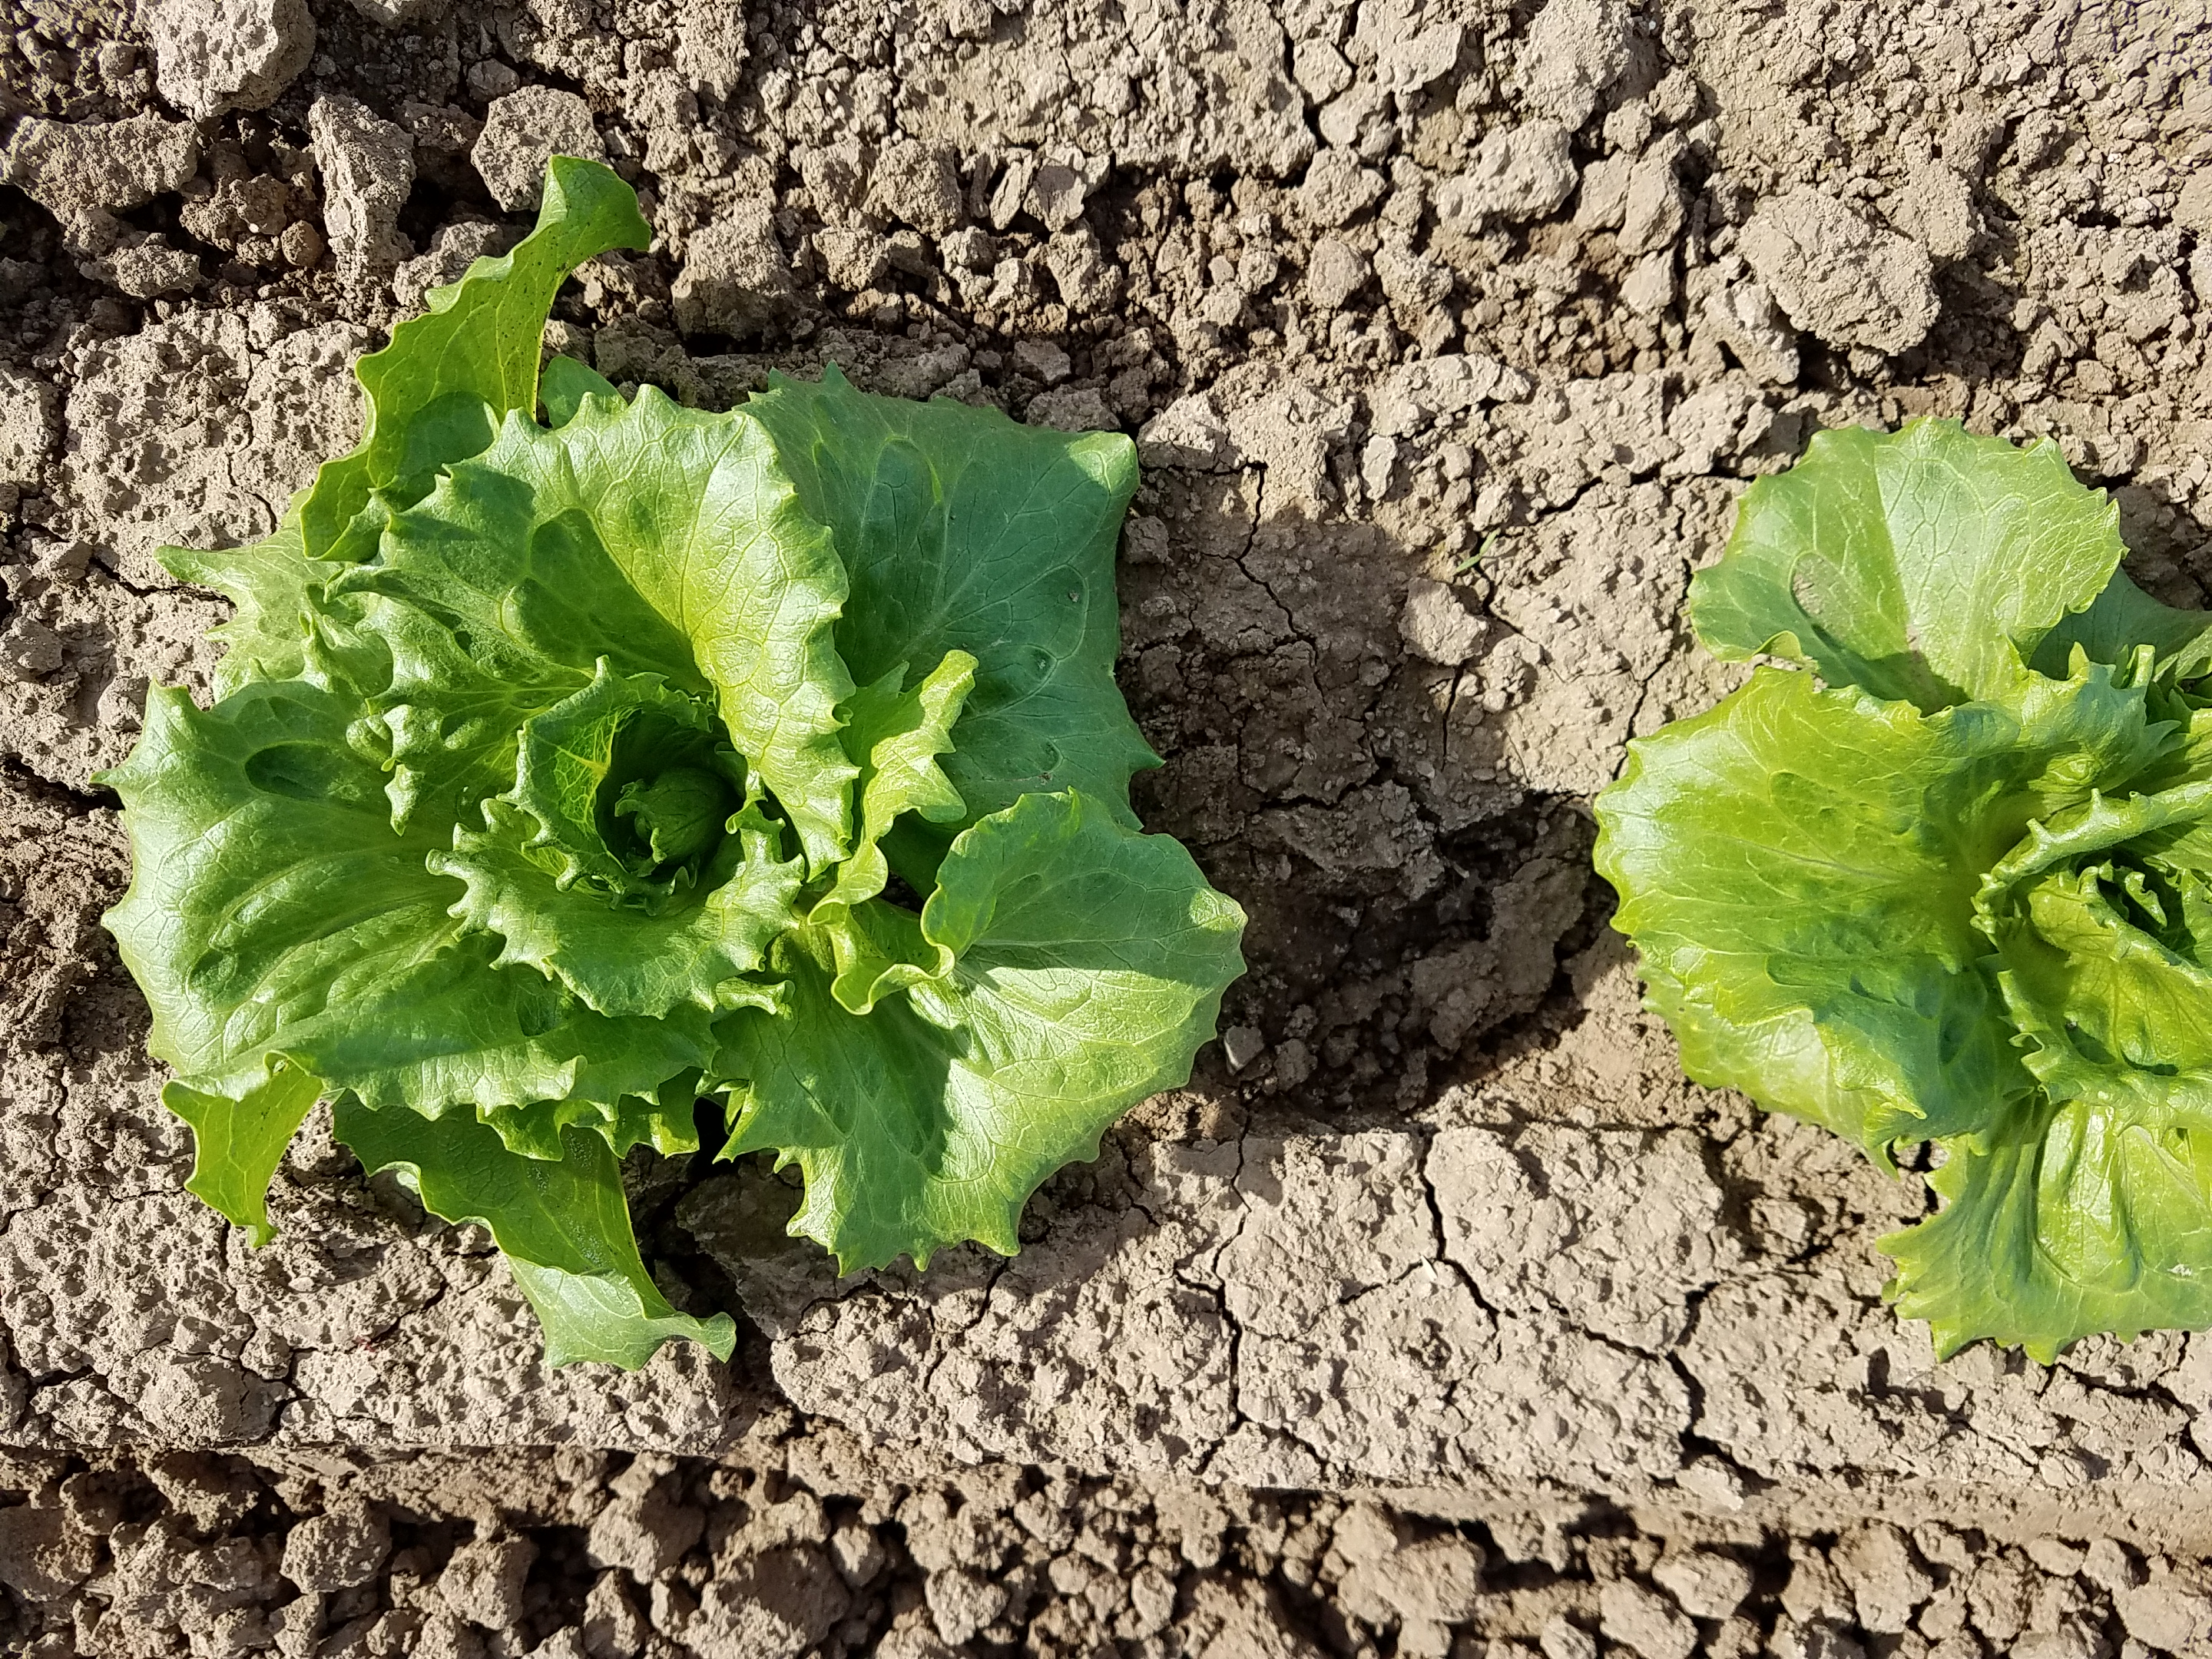
\includegraphics[width=1\linewidth]{./figures/problem-cutoff.jpg}
		\caption{The vegetation is cut off.}
		\label{fig:problem-cutoff}		
	\end{subfigure}%
	\caption[Common problems in field images]{These cases illustrate common problems encountered in image sets where the crop-line cannot be conclusively determined (\ref{fig:problem-cropline}) and the cutoff of vegetation (\ref{fig:problem-cutoff}). In the case where images contain a single image of crop the intended crop-line cannot be automatically determined. In the case where vegetation is cut off along the edges of the image shape analysis cannot be used, as otherwise the shape of the vegetation is distorted by the clean, straight edge. \\ \textit{Images source: Dr.~Mark Siemens, University of Arizona}}
\end{figure}



\subsection{Prepared Images}
The images acquired in the field are prepared using Adobe Photoshop\textsuperscript{\textregistered} to create test data for various scenarios:
\begin{itemize}
	\item{Rows of vegetation requiring thinning. This is the case where vegetation that would otherwise be classified as \textit{desired} is instead classified as \textit{undesired}, as its placement within the crop-line violates a placement rule. Typically, this would be the case where crop required thinning to achieve the minimum distance between plants.} This is achieved by duplicating an existing plant in the image and choosing a placement that will achieve that scenario.
	\item{Unwanted vegetation too close to wanted vegetation. This is the case where vegetation is identified as \textit{undesired}, but is left untreated due to the risk of treatment would pose to the crop.} This is achieved in two ways -- duplicating or moving an existing weed within the image and inserting a new weed image obtained elsewhere.
	\item{Debris in the image -- this is the case where non-vegetated matter appears in the image.}
\end{itemize}

\begin{figure}[H]
	\begin{subfigure}[h]{0.48\linewidth}
		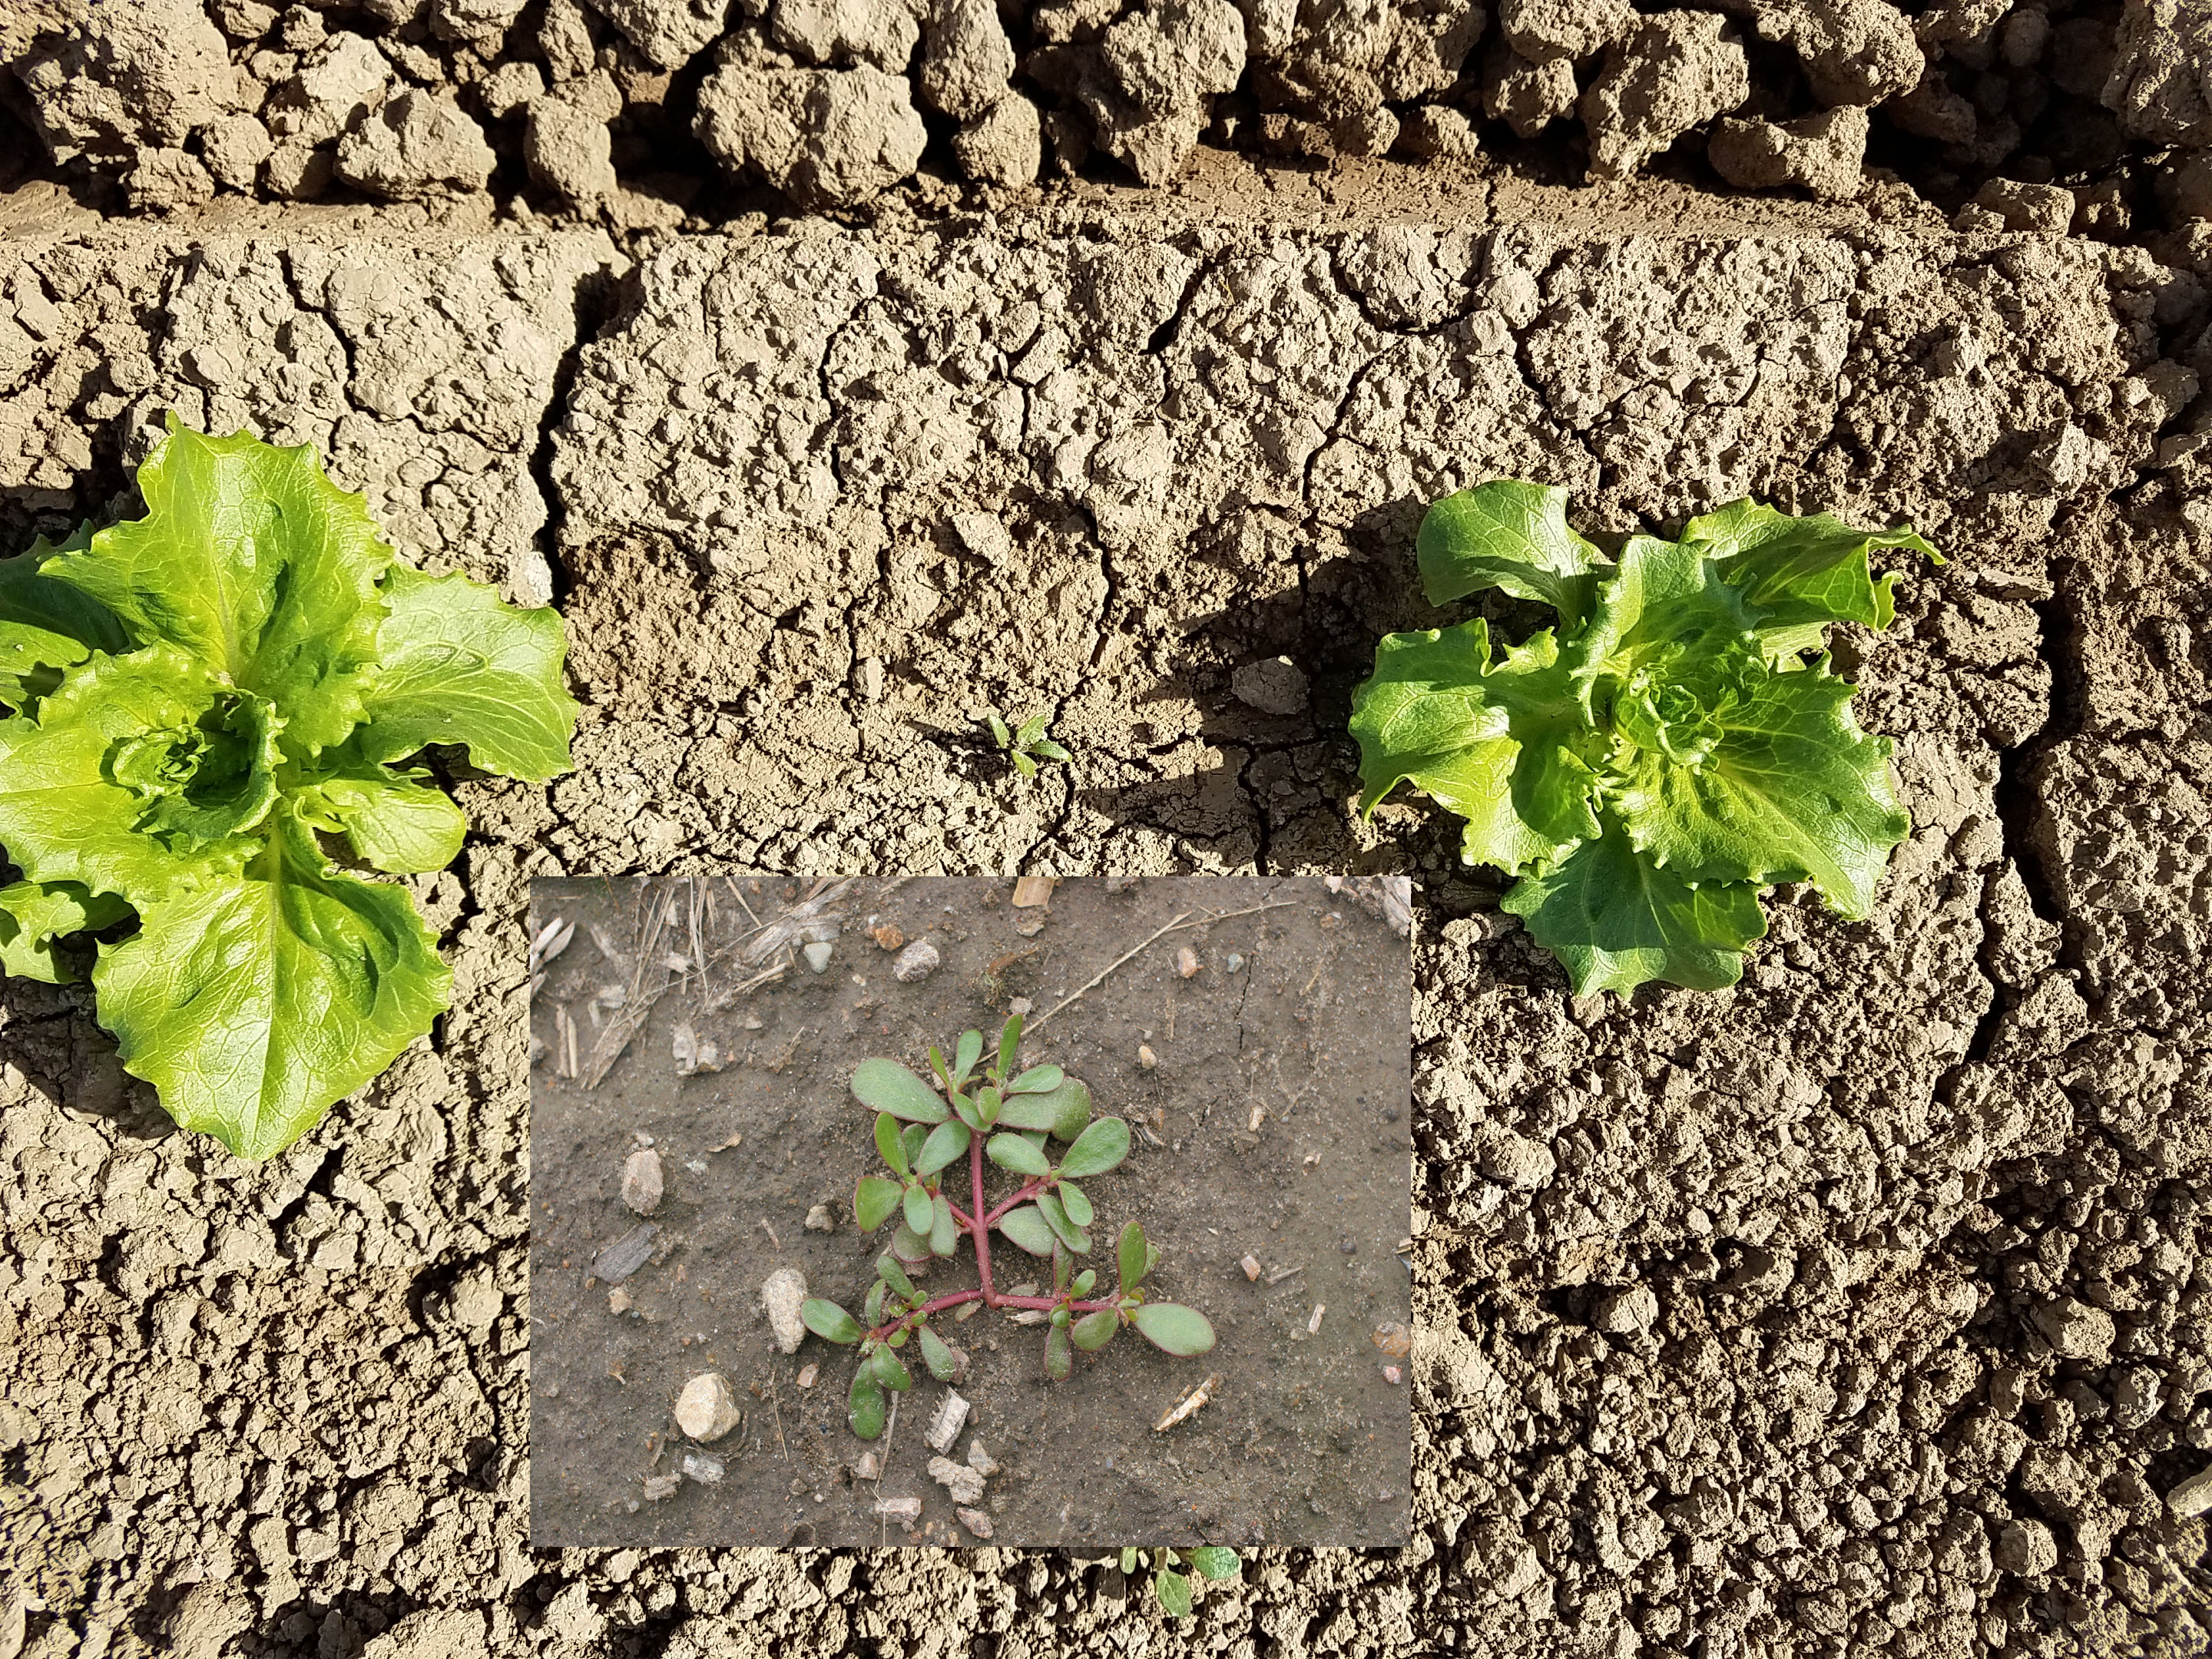
\includegraphics[width=1\linewidth]{./figures/with-purslane.jpg}
		\caption{Purslane (\textit Portulaca oleracea) inserted into the image.}
		\label{fig:prepared-weed}
	\end{subfigure}
	\hfill
	\begin{subfigure}[h]{0.48\linewidth}
		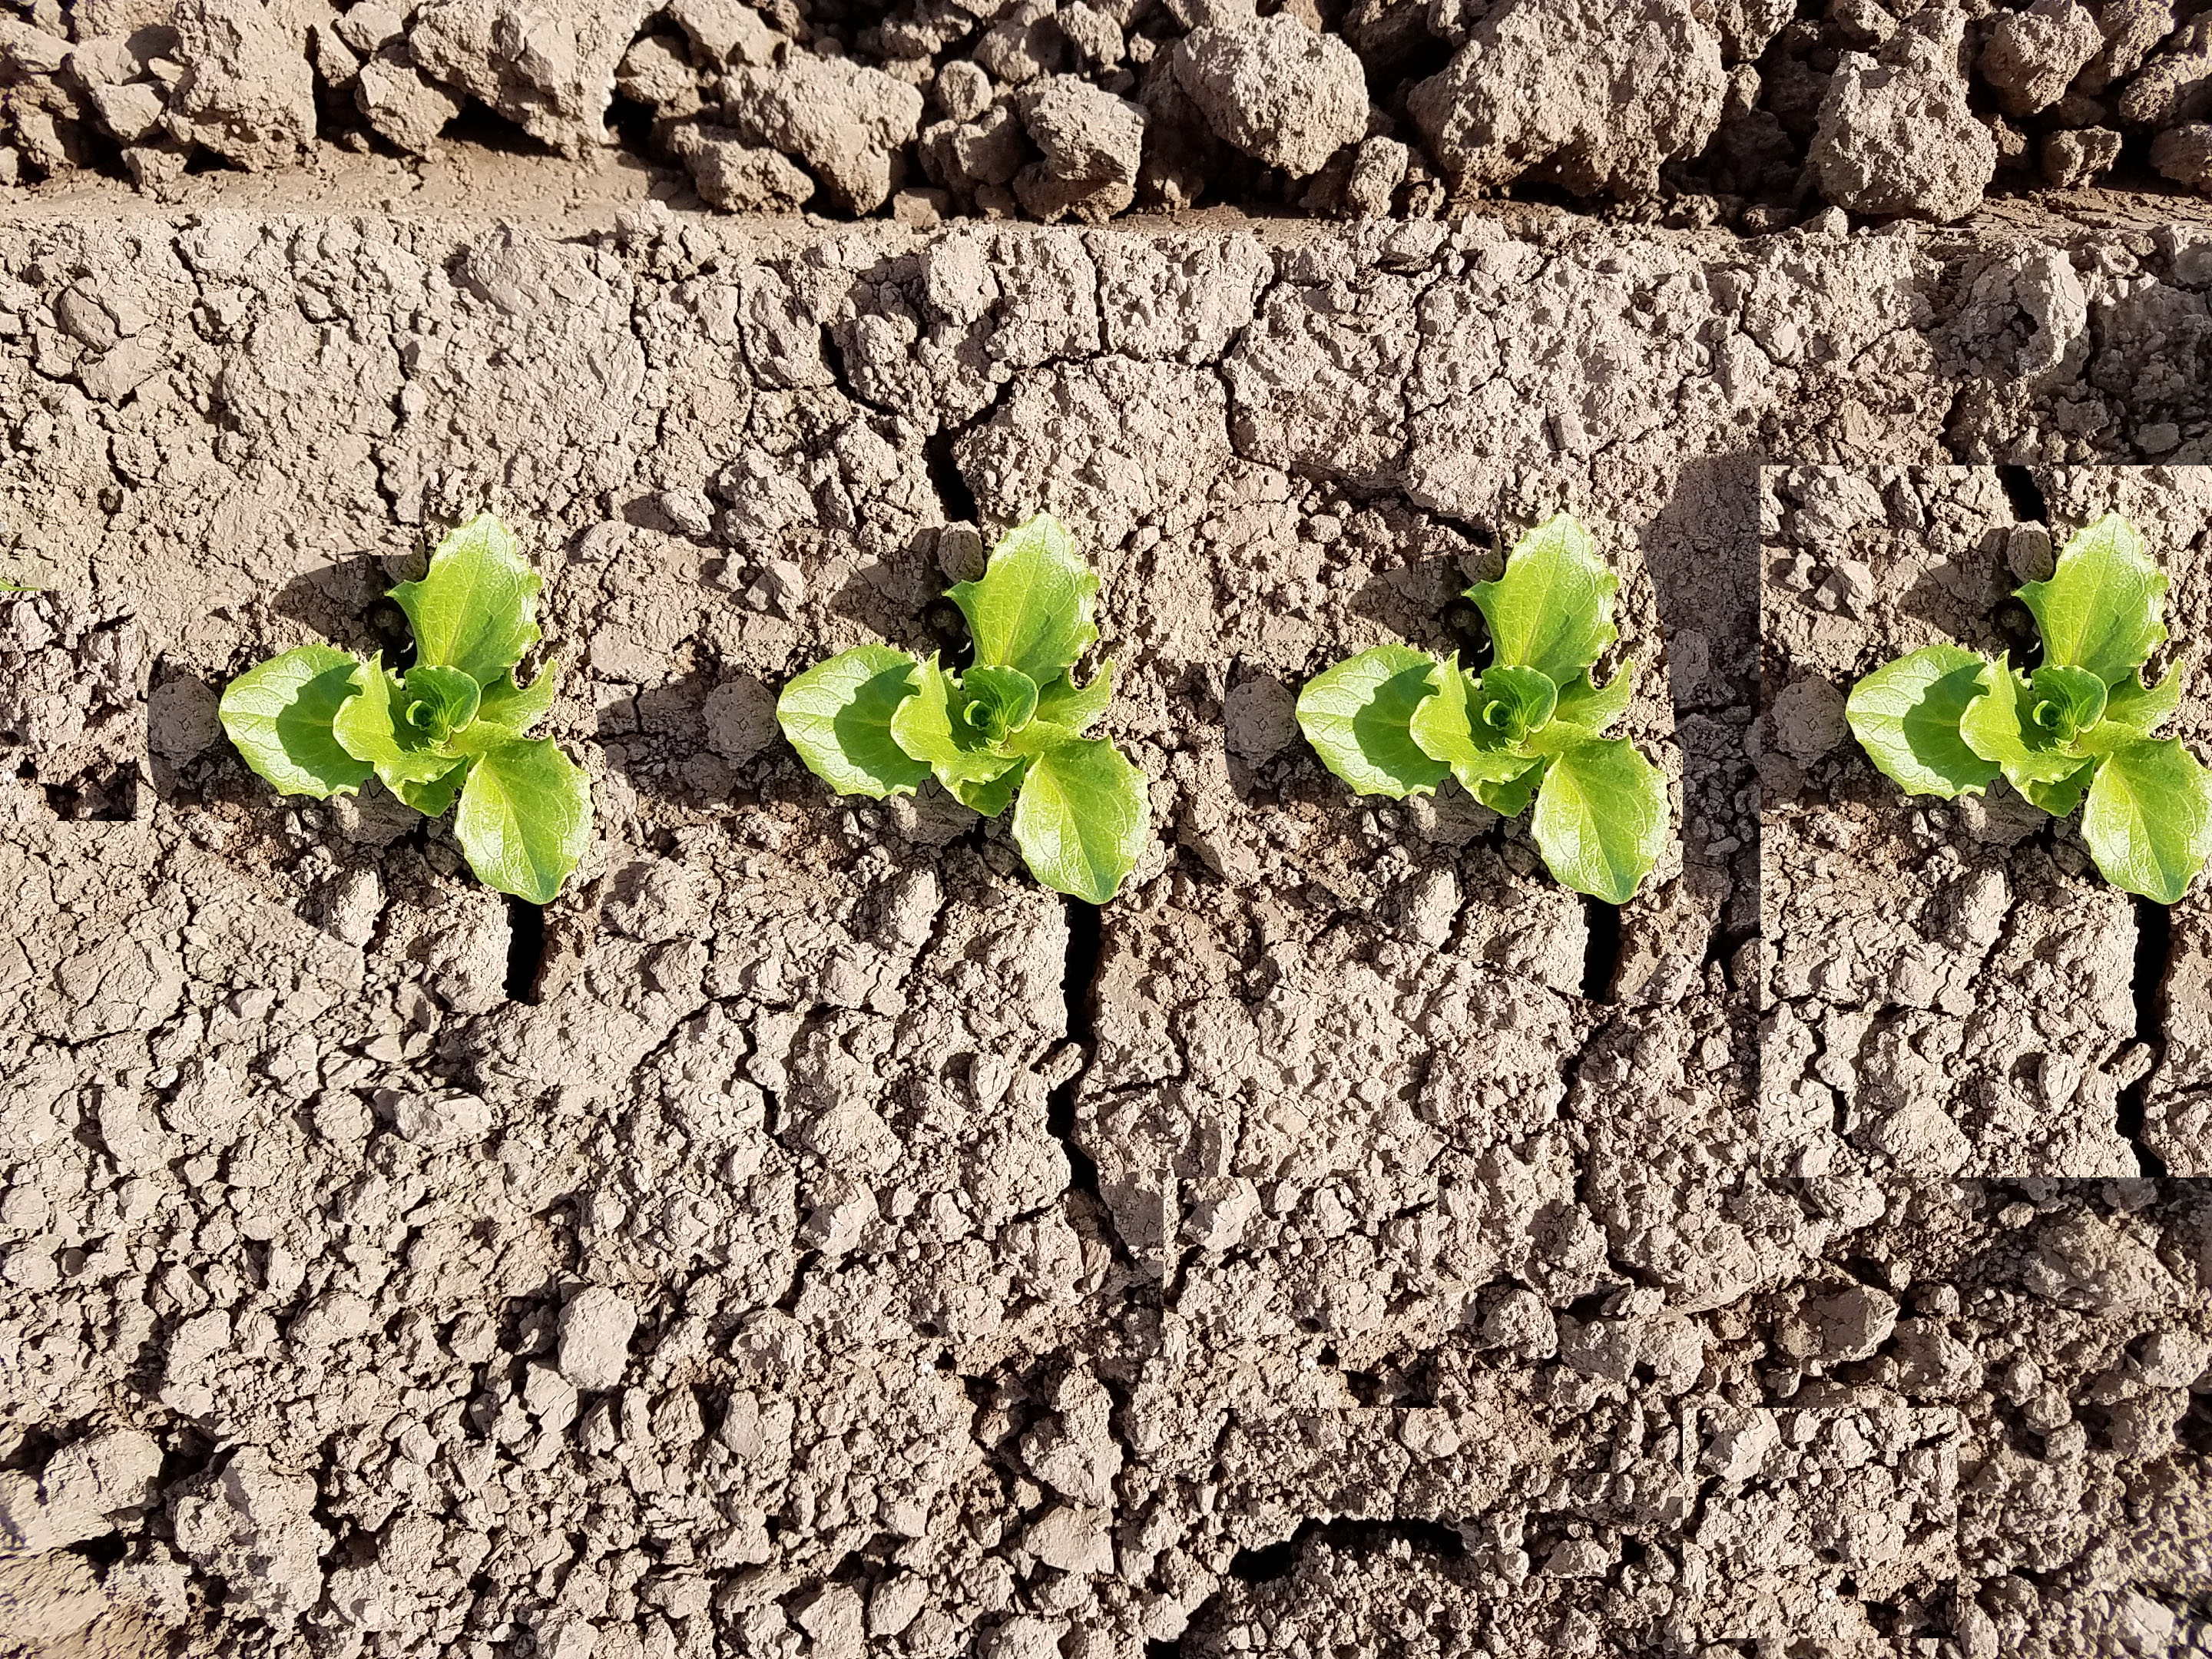
\includegraphics[width=1\linewidth]{./figures/thinning.jpg}
		\caption{Crop is replicated.}
		\label{fig:prepared-thinning}		
	\end{subfigure}%
	\caption[Prepared images]{Images acquired in the field are subsequently manipulated by either inserting images of weeds not already present (\ref{fig:prepared-weed}), or portions of the same image (\ref{fig:prepared-thinning}). Both cases are intended to present situations that should be handled by the classification algorithms. \\ \textit{Manipulated images of originals from Dr. Mark Siemens, University of Arizona}}
\end{figure}


Here, vegetation is placed within separate layers to create a composite image that shows the desired result. In Figure~\ref{fig:prepared-thinning}, a single lettuce plant is replicated several times to form an image that appears to be that of several plants. Notice the obvious seam in the lettuce plant on the right hand side of the image. As these pixels will be discarded early in image processing, they will have no effect on the current process as a whole, but may be a consideration if future processing considers factors such as the vegetation’s shadow.



\section{Approach To Classification}
The goal of this processing flow is to determine what each item within the image is and classify it as desired or undesired. Weeds are, of course, undesired, but crop plants can also be classified as \textit{undesired} in the case of thinning operations, so this document will use the term \textit{undesired} and \textit{weed} interchangeably. Vegetation in an image falls into one of these classifications:
\begin{itemize}
	\item{Desired, the crop}
	\item{Undesired, either crop that must be thinned or weeds that can be treated without crop damage}
	\item{Unknown, vegetation that cannot be confidently identified}
	\item{Ignored, vegetation that is too close to desired vegetation to be treated without crop damage}
\end{itemize}

Additionally, this work makes a few simplifying assumptions about the images:
\begin{itemize}
	\item{The crop line is approximately in the middle of the image.}
	\item{Crop is typically in roughly horizontal alignment (the centers will be with a few degrees of each other).}
	\item{Weed centers are typically not in horizontal alignment.}
	\item{Crop is typically much larger than weeds.}
\end{itemize}

These are not without exceptions. For instance, a weed may be in perfect aligment within a crop line and two other plants. Each of these observations, however, are used in classification. Take, for instance, the observation that crop tends to be much larger than weeds. If the size of an item is three times that of another, the smaller item is -- more likely than not -- a weed.

\section {Study Area}
The study was conducted at the University of Arizona Maricopa Agricultural Research Center (MAC)  as part of XXXXX

\section{Software Environment \& Source code}
Both commercial and open-source software were used in the development an operational aspects of this study. While the majority of the software (the operational portions responsible for image processing and classification) was written in Python, commercial packages were used for pre-processing. Additionally, R was used in visualization and analysis of classification results. Some of these components play a large enough role that they warrant special mention in various places throughout this document, but in-depth descriptions of them will not be made here. Likewise, this list is not exhaustive, as numerous libraries were used for a few functions, but included here. The complete source code for this project is available in this GitHub repository: \href{https://github.com/evan-mcginnis/weeds}{\textit {weeds}}. Images, both raw and processed, are far too large to be hosted with GitHub, and are available on request from the author.

All development was done on Windows 10 and Ubuntu 18.04.06 with analysis on the University of Arizona's \textit{High Performance Compute Cluster}.

{
% This avoids the document line spacing affecting the contents of the table
\setstretch{1.0}
\begin{longtable}{x{\dimexpr.20\columnwidth-2\tabcolsep}
                  x{\dimexpr.20\columnwidth-2\tabcolsep}
                  x{\dimexpr.5\columnwidth-2\tabcolsep}}
%\begin{hyphenrules}{nohyphenation}
    \caption{Software Used}\label{tab:software}  \\
\toprule
{\textbf{Component}} & {\textbf{Use}} & {\textbf{Comment}}
\tabularnewline
\midrule
    \endfirsthead
%%%%
    \caption{Software Used (cont.)}\label{tab:software}  \\
\toprule
{\textbf{Component}} & {\textbf{Use}} & {\textbf{Comment}}
\tabularnewline
\midrule
    \endhead
%%%%
\midrule[\heavyrulewidth]
\multicolumn{3}{r}{\footnotesize\itshape
                   Continued on the next page}
    \endfoot
%%%%
\bottomrule
    \endlastfoot
%%%%
		PyCharm 
		& Python IDE     
		& Commercial software for Python development
\tabularnewline\addlinespace
		Python 3.9     
		& Python runtime                    
		& Most software was written in python
\tabularnewline\addlinespace
		scikit-learn
		& Machine Learning     
		& Implementations for various ML techniques 
\tabularnewline\addlinespace
		OpenCV2 
		& Image Processing     
		& Machine Vision and Image Processing framework
\tabularnewline\addlinespace
		Numpy
		& Numeric Processing   
		& Python library
\tabularnewline\addlinespace
		Pandas 
		& Numeric Processing     
		& Python library
\tabularnewline\addlinespace
		PyQT5 
		& UI     
		& User Interface Framework for Python
\tabularnewline\addlinespace
		R 
		& Post Processing     
		& Statistical Software
\tabularnewline\addlinespace
		Plotly
		& Visualization     
		& Graphing libraries
\tabularnewline\addlinespace
		Adobe Lightroom
		& Color Correction     
		& Commercial software used for pre-processing
\tabularnewline\addlinespace
		Dronelink
		& UAV Control     
		& Commercial software used for planning \& control
\tabularnewline\addlinespace
		MongoDB
		& Image organization     
		& No-SQL database 
\tabularnewline\addlinespace
		Docker Container
		& Virtualization     
		& Virtual containers host database and web server
\tabularnewline\addlinespace
		Slurm
		& Workload     
		& Supercomputer workload management
\tabularnewline\addlinespace
		NGINX
		& Web Server     
		& Host HTTP API requests
\label{table:software}
\end{longtable}
}

\section{Workflow}
Images are processed following the workflow shown in Figure~\ref{fig:workflow}. Each step in this workflow will be discussed in subsequent sections.
\begin{figure}[H]
	\centering
	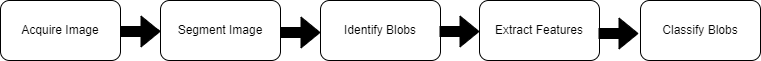
\includegraphics[width=1\linewidth]{./figures/workflow.drawio.png}
	\caption{Image processing workflow.}
	\label{fig:workflow}	
\end{figure}

\section{Acquire Image}
While the the processing step consists only of reading images from disk, actual acquisition was carried out in this study using a \href{https://www.dji.com/air-2s/specs} {DJI Mavic 2 S} drone with a 20 MP camera, followed by color correction. Each image acquisition was accompanied by an image of a \href{https://www.datacolor.com/spyder/products/spyder-checkr-photo/} {SpyderChecker 24} color calibration chart, and color correction was subsequently applied using Adobe Photoshop Lightroom Classic and custom calibration profiles created using the Spyder Checkr software. Raw sensor data was stored in Adobe Digital Negative (DNG) format before color correction and conversion to a compressed JPG format for the resulting images. The sensor data for each image was quite large, requiring 38.5 MB of storage, resulting in these requirements for the altitudes studied:

{\renewcommand{\arraystretch}{2}%

{
% This avoids the document line spacing affecting the contents of the table
\setstretch{1.0}
\begin{longtable}{x{\dimexpr.25\columnwidth-2\tabcolsep}
                  x{\dimexpr.35\columnwidth-2\tabcolsep}
                  x{\dimexpr.4\columnwidth-2\tabcolsep}}
%\begin{hyphenrules}{nohyphenation}
    \caption{Storage Requirements}\label{tab:storage}  \\
\toprule
{\textbf{AGL (meters)}} & {\textbf{DNG (Raw Sensor Data, MB)}} & {\textbf{Compressed (JPG, MB)}}
\tabularnewline
\midrule
    \endfirsthead
%%%%
    \caption{Storage Requirements (cont.)}\label{tab:storage}  \\
\toprule
{\textbf{AGL (meters)}} & {\textbf{DNG (Raw Sensor Data, MB)}} & {\textbf{Compressed (JPG, MB)}}
\tabularnewline
\midrule
    \endhead
%%%%
\midrule[\heavyrulewidth]
\multicolumn{3}{r}{\footnotesize\itshape
                   Continued on the next page}
    \endfoot
%%%%
\bottomrule
    \endlastfoot
%%%%
		2
		& XXX     
		& XXX
\tabularnewline\addlinespace
		5     
		& XXX                    
		& XXX
%\tabularnewline\addlinespace
\label{table:segmentation}
\end{longtable}
}

%
% I M A G E  S E G M E N T A T I O N
%
\section{Segmentation Image}
The portions of the images that did not contain pixels with vegetation present were the discarded by applying a visible light vegetation index to both isolate the vegetation and reduce the information content. This discards both the ground and debris while retaining the vegetation. These images were segmented using various visible light indices (\cite{Hunt2013-ih}, \cite{Hamuda2016-dw}). As this process is not the primary subject of this paper, it will be given only superficial mention here.  Various approaches to image segmentation are  summarized in Table \ref{table:segmentation}. 

{\renewcommand{\arraystretch}{2}%

{
% This avoids the document line spacing affecting the contents of the table
\setstretch{1.0}
% Example to span two pages
\begin{longtable}{x{\dimexpr.25\columnwidth-2\tabcolsep}
                  x{\dimexpr.35\columnwidth-2\tabcolsep}
                  x{\dimexpr.4\columnwidth-2\tabcolsep}}
%\begin{hyphenrules}{nohyphenation}
    \caption{Visible light indices}\label{tab:example}  \\
\toprule
{\textbf{Index}} & {\textbf{Formula}} & {\textbf{Comment}}
\tabularnewline
\midrule
    \endfirsthead
%%%%
    \caption{Visible light indices (cont.)}\label{tab:example}  \\
\toprule
{\textbf{Index}} & {\textbf{Formula}} & {\textbf{Comment}}
\tabularnewline
\midrule
    \endhead
%%%%
\midrule[\heavyrulewidth]
\multicolumn{3}{r}{\footnotesize\itshape
                   Continued on the next page}
    \endfoot
%%%%
\bottomrule
    \endlastfoot
%%%%
		Triangular Greenness
		& \begin{minipage}[t]{0.3\textwidth}
			$R_{green} - \alpha R_{red} - \beta R_{blue}\\ \alpha = \frac {2(\lambda_{blue} - \lambda_{green})} {(\lambda_{blue} - \lambda_{red})}\\ 
		    	\beta = \frac {2(\lambda_{green} - \lambda_{red})} {(\lambda_{blue} - \lambda_{red})} $
		   \end{minipage}     
		& Corrects for camera calibration using the peak sensitivity
\tabularnewline\addlinespace

		Normalized Difference     
		& $128 * \left( \left( \frac {(G - R)} {(G + R)} \right) + 1 \right) $                    
		& The NDI index produces a near-binary image. 
\tabularnewline\addlinespace

		Excess Green      
		& \begin{minipage}[t]{0.3\textwidth}
			$R = \frac {R} {R_{max}}\\ G = \frac {G} {G_{max}}\\ B = \frac {B} {B_{max}}$ 
		   \end{minipage}
		& ExG provided a clear contrast between plants and soil 
\tabularnewline\addlinespace

		Excess Red      
		& $1.3 R - G$ 
		& inspired by the fact that there are 4\% blue, and 32\% green, compared with 64\% red cones in the retina of the human eye
\tabularnewline\addlinespace

		Color Index of Vegetation Extraction      
		& $0.441 R - 0.811 G + 0.385 B + 18.78745$
		& This method was proposed to separate green plants from soil background in order to evaluate the crop growing status.
\tabularnewline\addlinespace

		Excess Green - Excess Red   
		& $ExG - ExR$ 
		& ExG used to extract the plant region and ExR used to eliminate the background noise (soil and residue) where green–red material (stems, branches, or petioles) may exist
\tabularnewline\addlinespace

		Normalized Green-Red Difference    
		& $\frac {(G - R)} {(G + R)}$ 
		& The method of NGRDI was used to overcome the differences in exposure settings selected by the digital camera when acquiring aerial photography of the field. 
\tabularnewline\addlinespace

		Vegetative Index      
		& $\frac {G} {R^aB^{(1-a)}}, a = 0.667$ 
		& VEG has a significant advantage because it is robust to lighting change.
\tabularnewline\addlinespace

		Com1   
		& $ExG + CIVE + ExGR + VEG$ 
		& High computational cost --- does not perform well in high or low light levels
\tabularnewline\addlinespace

		Modified Excess Green      
		& $1.262G - 0.884R = 0.311B$ 
		& Does not perform well in high or low light levels. 
\tabularnewline\addlinespace

		Combined Indices 2      
		& $0.36ExG + 0.47CIVE + 0.17VEG$ 
		& Uses weighting factors to emphasize strengths of various approaches
%\tabularnewline\addlinespace
\label{table:segmentation}
\end{longtable}
}


These indices are used to create a mask that is then applied to the original source image to permit vegetation to show while masking details that are not relevant (ground pixels, stones, and other items that may appear in field conditions) The intent here is to remove all pixels that are not relevant to the task of distinguishing between crop and weed while leaving the vegetated pixels unmanipulated.

\begin{figure}[H]
	\centering
	\begin{subfigure}[h]{.30\textwidth}
	  \centering
	  \includegraphics[width=1\linewidth]{figures/original.jpg}
	  \caption{Field view of lettuce and weed}
	  \label{fig:original}
	\end{subfigure}
	\begin{subfigure}[h]{.30\textwidth}
	  \centering
	  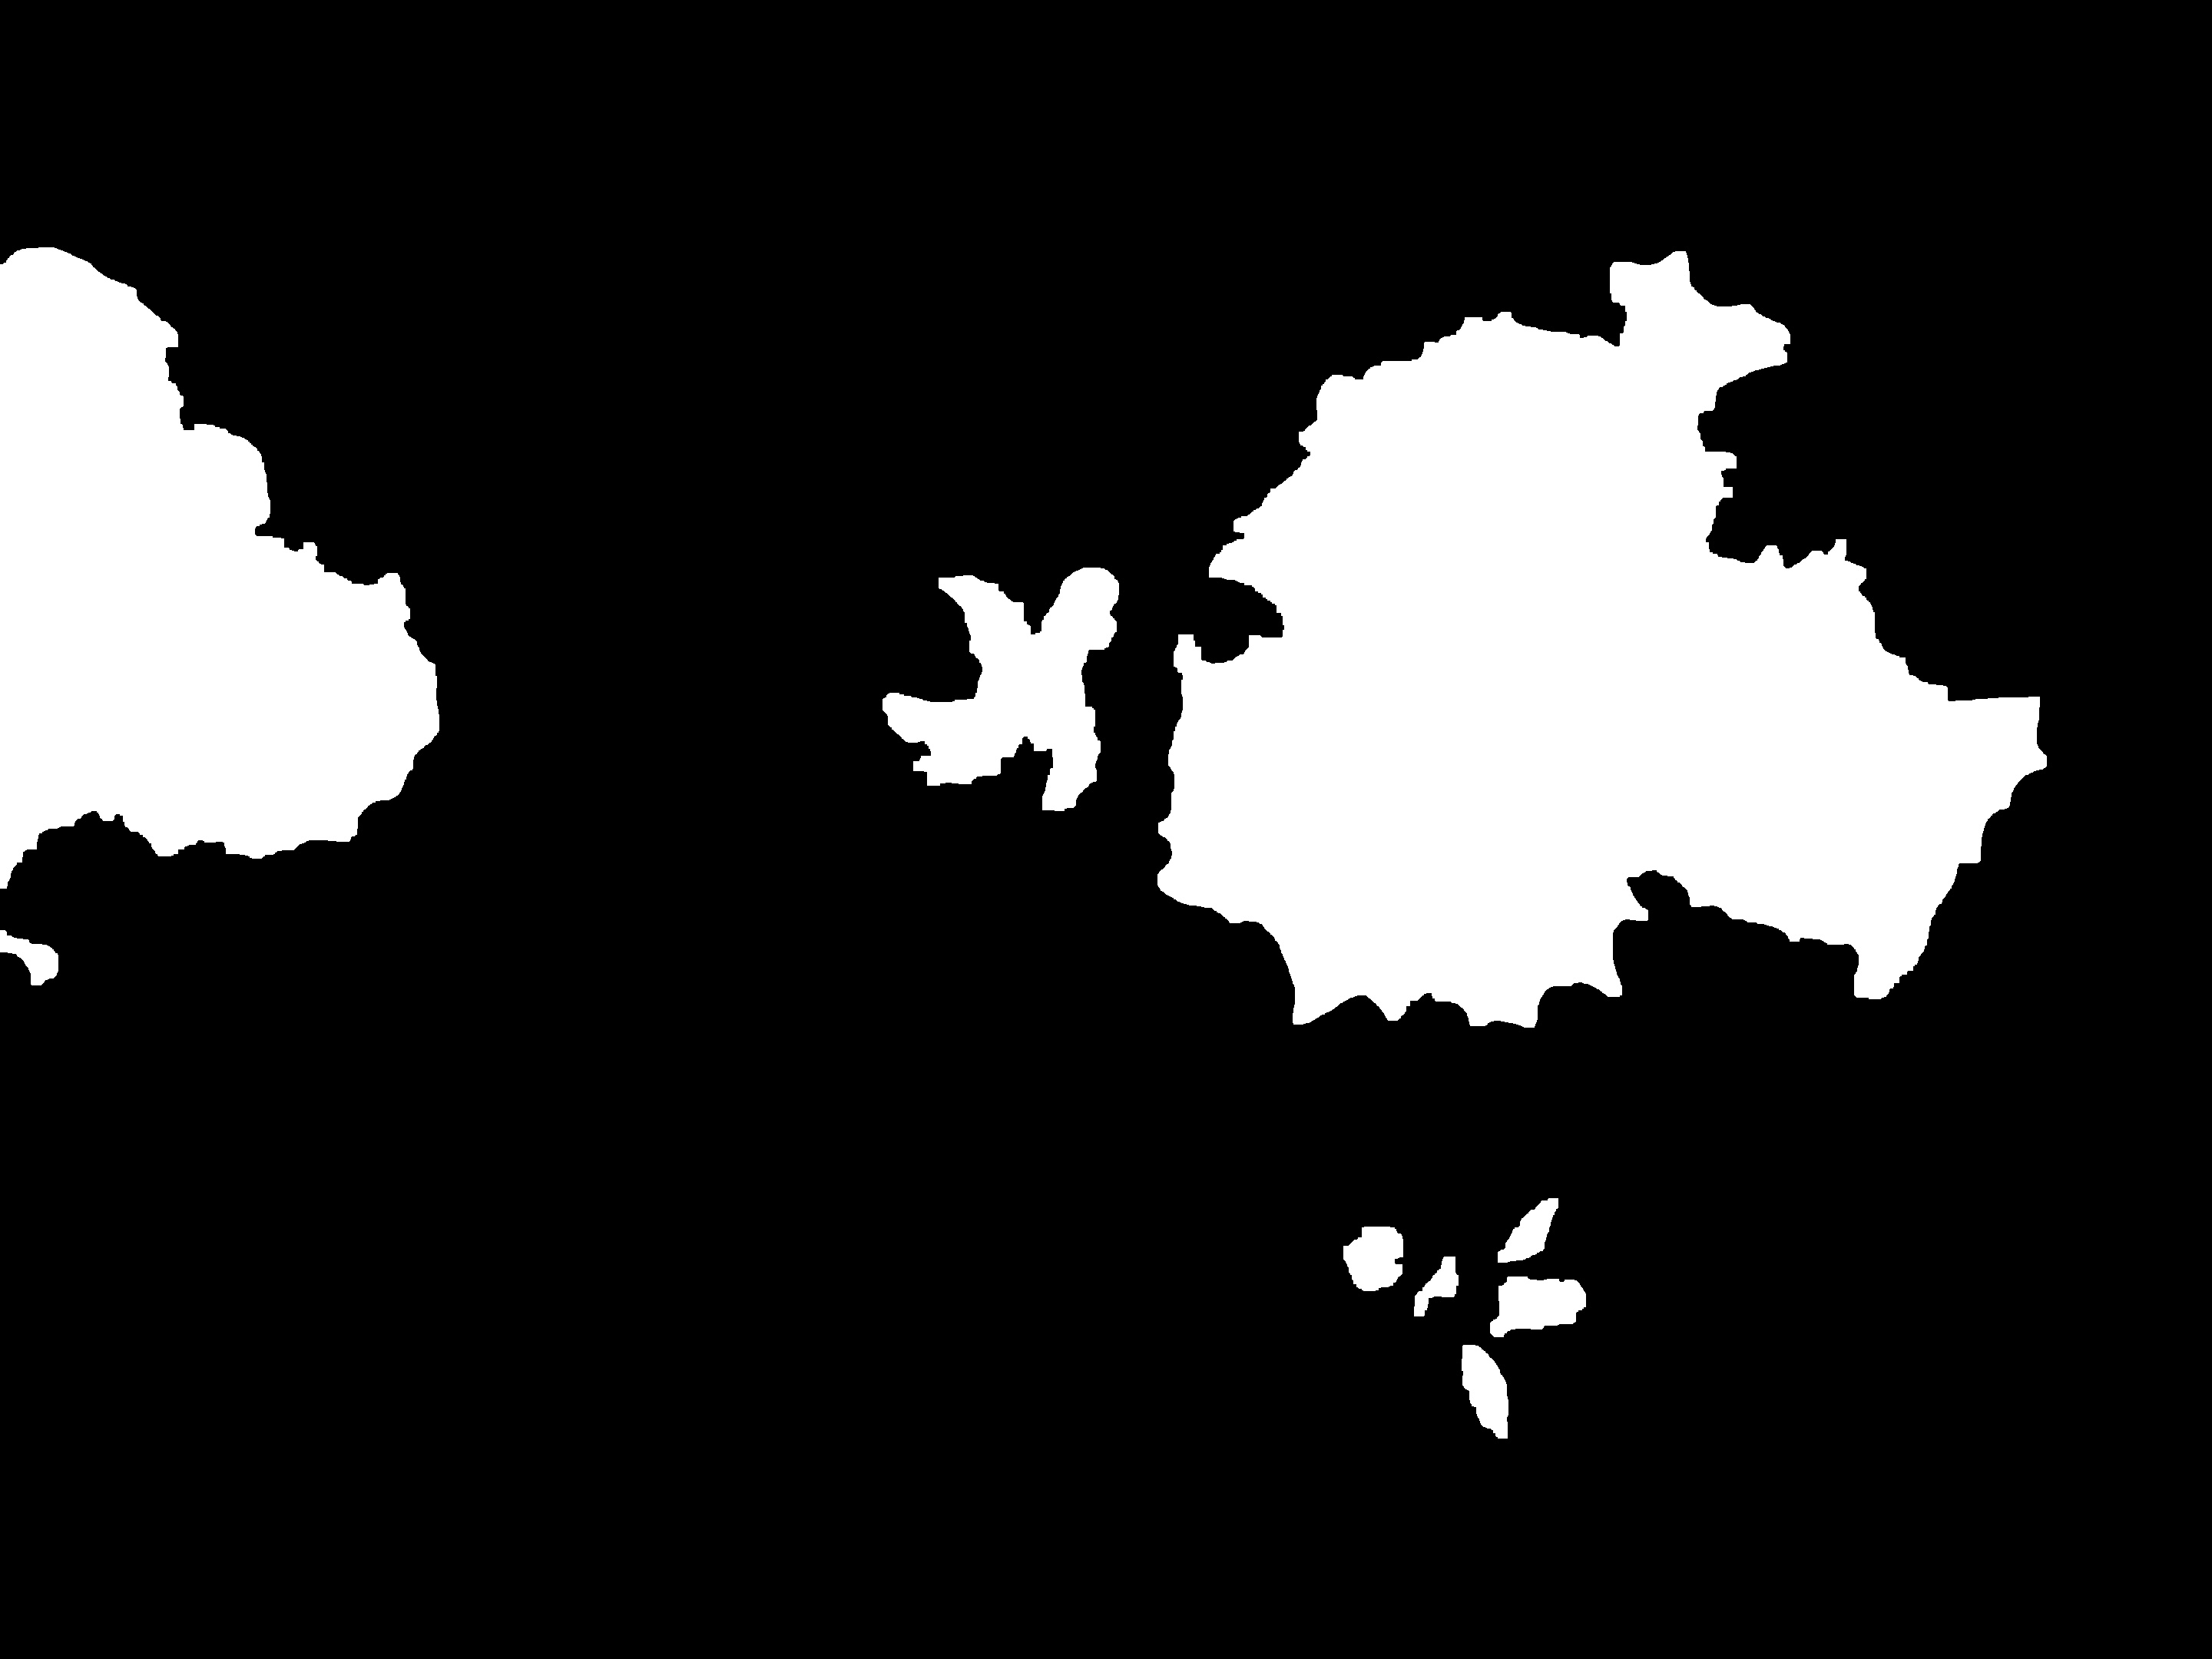
\includegraphics[width=1\linewidth]{figures/original-mask.jpg}
	  \caption{Mask produced with NDI}
	  \label{fig:mask}
	\end{subfigure}
	\begin{subfigure}[h]{.30\textwidth}
	  \centering
	  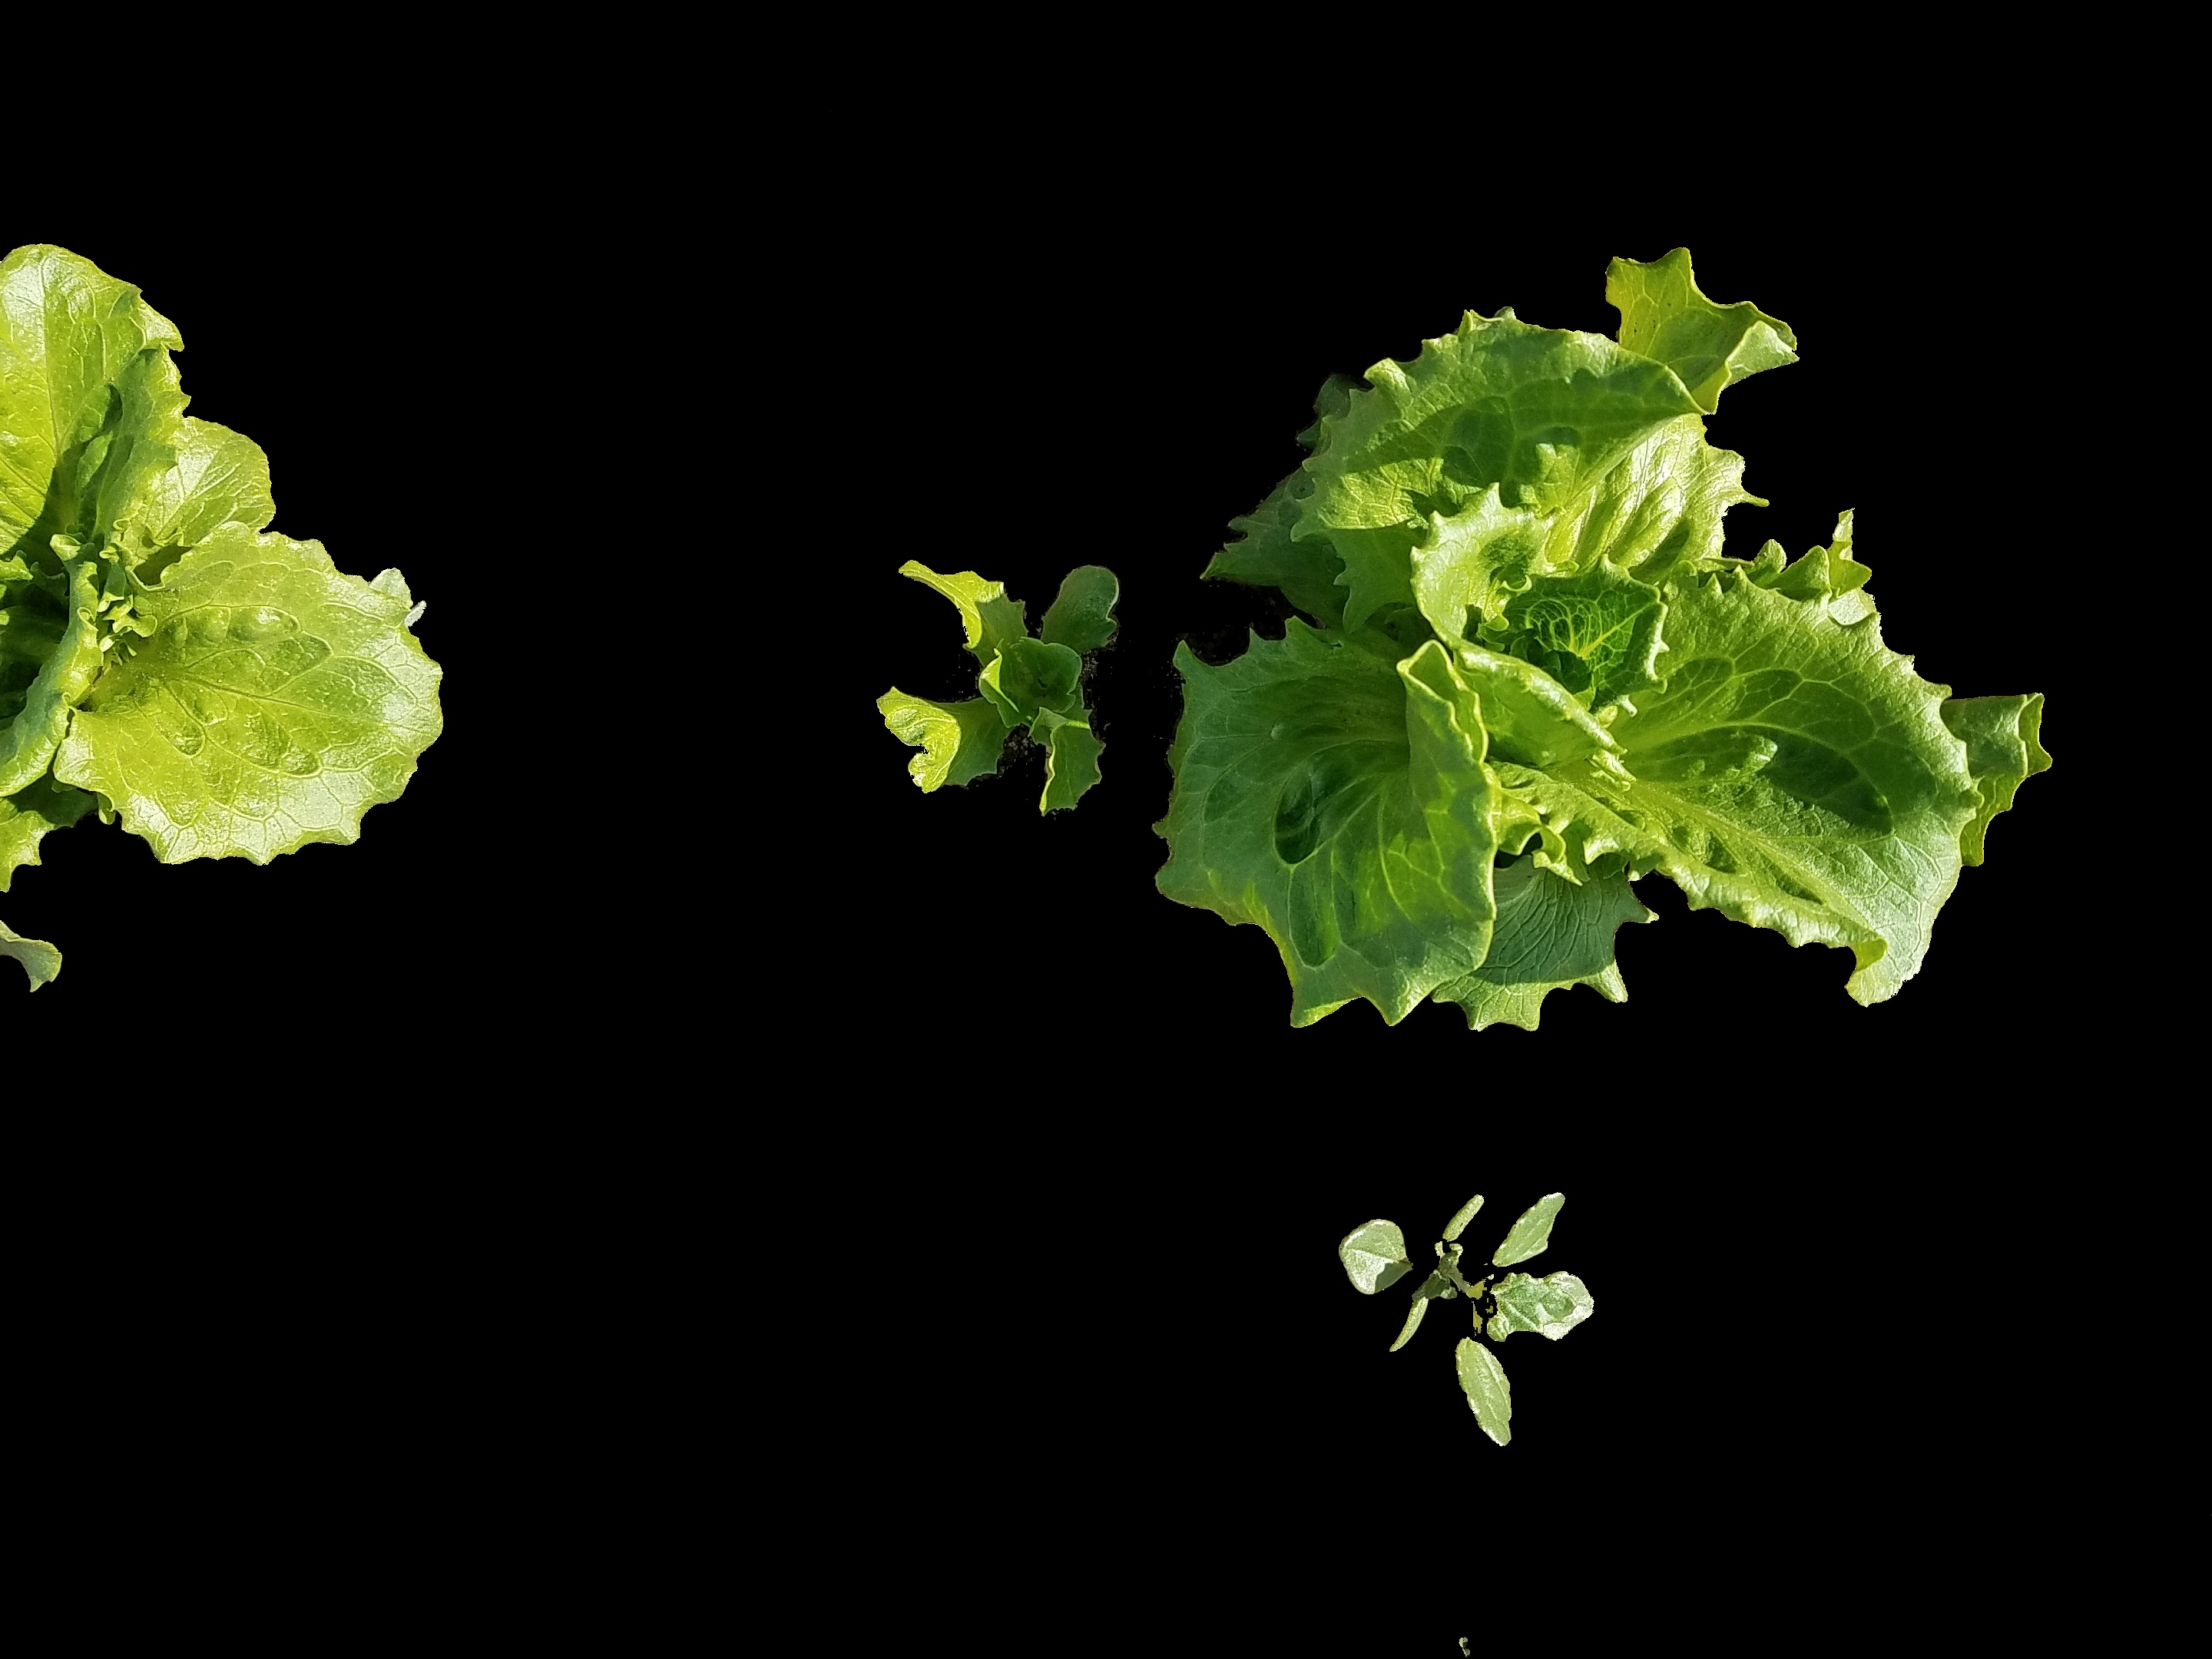
\includegraphics[width=1\linewidth]{figures/original-masked.jpg}
	  \caption{After applying mask}
	  \label{fig:original-masked}
	\end{subfigure}
	\caption[Before and after segmentation]{Before and after segmentation. Note the absence of the stems seen in the weed in the lower portion of~\ref{fig:original-masked} -- this is made a bit more obvious with a close examination of the mask shown in~\ref{fig:mask}. The lack of stems will lead to a single plant being identified as multiple plants, but has no effect on the classification using the features identified as significant.}
	\label{fig:segmentation}
\end{figure}
The segmented image has discarded ground pixels while retaining most of the pixels that will be used, but a close examination reveals that pixels in the stems of the weed are also eliminated, as they are less green than the rest of the plant. This effect is even more pronounced when segmenting images of weed that do not contain green stems as would be seen in the red stems seen in \textit{Portulaca oleracea} (Purslane). While they are not eliminated, pixels in the area of the deep shadows of the vegetation may affect attempts to classify objects based on color attributes. Unfortunately, the band of color featured in the stems (red) is frequently found in the background (soil), so attempts to make the stems appear in the masked image are problematic, as this solution tends to bring allow unwanted ground pixels in the final image that contain hues found within the stems. Likewise, immature vegetation where stems are not sufficiently green will not appear in the final image. Fortunately, both of these cases do not appear to have an appreciable effect on the classification. For the purposes of this paper, images will use the \textit{Normalized Difference Index} (NDI) segmentation approach (see Table~\ref{table:segmentation} for this formula). This process results in image data with only two sets of values: RGB values of zero where there is no vegetation and the original RGB values for pixels containing vegetation.

\section{Blob Identification}
Segmented images yield images with only vegetated pixels. Single items within those images are often called (somewhat generically) \textit{blobs}, and as that is the term generally used by the OpenCV software libraries used for image processing, that is the term adopted for this document. Blobs are identified as an object requiring classification, but not yet classified. Figure~\ref{fig:original-masked} is an example of this concept. This image shows eight blobs that can be classified: three lettuce plants and a single weed plant that appears as five plants in the final image.

\section{Feature Extraction}
Once the vegetation is isolated and blobs identified, various features can be extracted for subsequent use in classification. These features include position-independent characteristics such as shape, hue, and textural characteristics as well as position-dependent features such as where a plant resides relative to the crop-line.  

\subsection{Shape Characteristics}
The shape parameters considered in this analysis are expressions describing the perimeter of the plant. The shape formulae used to extract the various shape features are given in Table~\ref{tab:shape-formulae}, but some concepts and formulae warrant further explanation.

\subsubsection{Bounding Box and Convex Hull}
An object can be said to have rectangular box of minimum size that completely encloses the object, commonly termed the \textit{bounding box}. The box placed around the object without regard for orientation -- that is, the placement makes no attempt to align the edges of the box with the edges of the image, so it may appear tilted at normal viewing angles. The \textit{convex hull}, likewise, is a convex shape with straight lines and of minimum size that completely encloses the object. 

\subsubsection{Area \& Size Ratio}
The area of the plant in the image is the number of pixels with non-zero values. The relative area of two plants can then be compared. For instance, if a plant is $1/3$ the size of the largest plant in the image it is more likely than not a weed. This ratio is highly dependent on the development phase of the crop, as the reverse could be true for crop just emerging compared to much larger weeds. For the classification purposes presented here, the larger item is presumed to be crop.

\subsubsection{Length/Width Ratio}
\label{sec:width-length-ratio}
The ratio of width to length is not -- as the name might imply -- a simple ratio of two measurements, but is expressed as:
\begin{equation}
S = 
	\begin{bmatrix}
	Var(X) & Cov(XY) \\[0.3em]
	Cov(XY) & Var(Y) \\[0.3em]
	\end{bmatrix},
\lambda = \frac {eig_{1}(S)} {eig_{2}(S)}
\end{equation}
Where $eig_{1}(S)$ and $eig_{2}(S)$ are the maximum eigenvalues of the matrix $S$, with $\lambda$ representing the ratio. (\cite{Lin2017-xq}) The X and Y positions refer to an object's perimeter -- the boundary between an object's edge and the background.

% Begin table of shape equations
\begin{longtable}{x{\dimexpr.15\columnwidth-2\tabcolsep}
                  x{\dimexpr.425\columnwidth-2\tabcolsep}
                  x{\dimexpr.425\columnwidth-2\tabcolsep}}
%\begin{hyphenrules}{nohyphenation}
    \caption{Shape Features}\label{tab:shape-formulae}  \\
\toprule
{\textbf{Feature}} & {\textbf{Formula}} & {\textbf{Comment}}
\tabularnewline
\midrule
    \endfirsthead
%%%%
    \caption{Shape Features (cont.)}\label{tab:shape-formulae}  \\
\toprule
{\textbf{Feature}} & {\textbf{Formula}} & {\textbf{Comment}}
\tabularnewline
\midrule
    \endhead
%%%%
\midrule[\heavyrulewidth]
\multicolumn{3}{r}{\footnotesize\itshape
                   Continued on the next page}
    \endfoot
%%%%
\bottomrule
    \endlastfoot
%%%%
		Perimeter
		& \begin{minipage}[t]{0.3\textwidth}
			$\sum_{i=1} ^{N-1}\left|X_1 - X_{i+1}\right| $
		   \end{minipage}     
		& Count of pixels forming the boundary of an object
\tabularnewline\addlinespace

		Major/Minor Axis     
		& $\sqrt{(x_2 - x_1)^2 + (y_2 - y_1)^2} $                    
		& Major axis is the longest line that can be drawn through the object. Minor axis is the longest line that can be drawn through the object such that the line remains perpindicular to the major axis.
\tabularnewline\addlinespace

		Compactness      
		& \begin{minipage}[t]{0.3\textwidth}
			$\frac{4\pi * area}{(perimeter)^2}$ 
		   \end{minipage}
		& Ratio of an object's area to the area of a circle having the same perimeter 
\tabularnewline\addlinespace

		Elongation      
		& $\frac{width_{bounding}}{length_{bounding}}$ 
		& Ratio of the width of the object's bounding box to its width
\tabularnewline\addlinespace

		Eccentricity      
		& $\frac{length_{minor}}{length_{major}}$
		& Ratio of the minor to major axis
\tabularnewline\addlinespace

		Convexity   
		& $\frac{convex~perimeter}{perimeter}$ 
		& Ratio of the convex perimeter to the perimeter.
\tabularnewline\addlinespace

		Solidity    
		& $\frac{area}{convex~area}$ 
		&  Ratio of an object's area to its convex area. 
\tabularnewline\addlinespace

		Circularity    
		& $\frac{4\pi * area}{convex~perimeter}$ 
		& Ratio of an object's area to its convex perimeter. 
\tabularnewline\addlinespace


		Shape Index    
		& $\alpha = \frac {e} {4 \sqrt{A}}$ 
		&  Relationship between an object's perimeter and its area
\tabularnewline\addlinespace

		Width/Length Ratio
		& \begin{minipage}[h]{0.10\textwidth}
			\begin{eqnarray*}
				S = 
				\begin{bmatrix}
					Var(X) & Cov(XY) \\[0.10em]
					Cov(XY) & Var(Y) \\[0.10em]
				\end{bmatrix}
			\lambda = \frac {eig_{1}(S)} {eig_{2}(S)}
			\end{eqnarray*}
		  \end{minipage}
		& See section~\ref{sec:width-length-ratio}
\tabularnewline\addlinespace

\label{table:shape-formulae}
\end{longtable}
}
% End table of shape equations

%
% C O L O R
%
\subsection{Color}
\subsubsection{Hue \& Saturation}
The terms {\it color} and {\it hue} are often used interchangeably, and while this is mostly true, hue refers to the dominant color family. In this case, the image is converted to the Hue, Saturation, and Intensity {\it HSV} colorspace and the mean value for the hue of a blob's pixels is taken. The saturation of a color expressed by a component of the Hue, Saturation, and Intensity ({\it HSI}) colorspace and the mean value for the saturation of a blob's pixels is taken. (\cite{Forsyth2012-hy})

\subsubsection{YIQ}
The YIQ model of color used by the NTSC color TV system. Y represents the luma information, I and Q the chrominance information. The processing employed here is to convert the image to the YIQ color space and take the mean value for the I, or in-phase component for the blob's pixels. (\cite{MathWorks_undated-jg})
%\begin{figure}[h!]
%	\centering
%	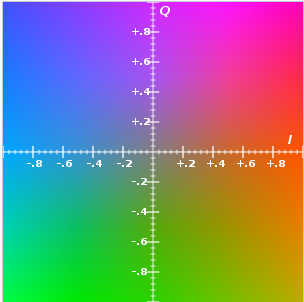
\includegraphics[width=0.4\linewidth]{./figures/yiq.png}
%	\caption{YIQ (Reproduced from\protect\cite{Various_undated-cz})}
%	\label{fig:yiq}
%\end{figure}
The $I$ component is the feature of interest here, and conversion of RGB to YIQ is achieved with this transformation:
\begin{equation}
	\begin{bmatrix}
	Y \\[0.3em]
	I \\[0.3em]
	Q \\[0.3em]
	\end{bmatrix}
	\approx
	\begin{bmatrix}
	0.299 & 0.587 & 0.114 \\[0.3em]
	0.5959 & -0.2746 & -0.3213\\[0.3em]
	0.2115 & -0.5227 & 0.3112 \\[0.3em]
	\end{bmatrix}
	\begin{bmatrix}
	R \\[0.3em]
	G \\[0.3em]
	B \\[0.3em]
	\end{bmatrix}	
\end{equation}

\subsubsection{HSI \& HSV}
\parencite[p.~84]{Forsyth2012-hy}
\subsubsection{CIElab}
\subsubsection{YCBCR}
The ECMA report on the JPG file format gives this transformation for RGB to YCBCR:
\nocite{Ecma2019-yo}
\begin{equation}
	\begin{bmatrix}
	Y \\[0.3em]
	C_b \\[0.3em]
	C_r \\[0.3em]
	\end{bmatrix}
	\approx
	\begin{bmatrix}
	0.2126 & 0.7152 & 0.0722 \\[0.3em]
	-0.1146 & -0.3854 & 0.5 \\[0.3em]
	0.5 & -04542. & -0.458 \\[0.3em]
	\end{bmatrix}
	\begin{bmatrix}
	R \\[0.3em]
	G \\[0.3em]
	B \\[0.3em]
	\end{bmatrix}	
\end{equation}

\subsection{Textural}
Textural descriptors of a object are formal expressions of the relationship pixel values have with one another, reducing a tactile experience to a numerical one. Here, the analysis technique employed is \textit{Grey-level Co-occurrence Matrix} (GLCM) (\cite{Haralick1973-gr}, \cite{Hall-Beyer2017-nx}). Haralick describes the analysis of an image that has been converted to greyscale values to note the relationship. Table~\ref{tab:glcm-formulae} details the subset that will be used in this analysis. The term \textit{grey-level} implies that the use of the co-occurrence matrix will be limited to greyscale images. Instead, the co-occurrence matrix will also be computed for each of the channels in the YIQ, RGB, CIELab, HSI, HSV, YCBCR colorspaces using the equations detailed in Table~\ref{tab:glcm-formulae}. GLCM attributes have two factors that relevant to this problem space: the distance of a pixel  considered to be a \textit{neighbor} and the angle of the relationship. Neighbor distance can be thought of as what is considered to adjacent -- the pixel immediately beside the one in question, or further away. This study considers pixels immediately adjacent to be neighbors. While images of crops are often gathered in an orderly manner along a row such that orientation is maintained, the vegetation is not so orderly. \citeauthor*{Haralick1973-gr} discuss this, suggesting that the mean of calculations be used instead of the individual angles.
\begin{longtable}{x{\dimexpr.15\columnwidth-2\tabcolsep}
                  x{\dimexpr.225\columnwidth-2\tabcolsep}
                  x{\dimexpr.625\columnwidth-2\tabcolsep}}
%\begin{hyphenrules}{nohyphenation}
    \caption{GLCM Formulae}\label{tab:glcm-formulae}  \\
\toprule
{\textbf{Feature}} & {\textbf{Formula}} & {\textbf{Comment}}
\tabularnewline
\midrule
    \endfirsthead
%%%%
    \caption{GLCM Features (cont.)}\label{tab:glcm-formulae}  \\
\toprule
{\textbf{Feature}} & {\textbf{Formula}} & {\textbf{Comment}}
\tabularnewline
\midrule
    \endhead
%%%%
\midrule[\heavyrulewidth]
\multicolumn{3}{r}{\footnotesize\itshape
                   Continued on the next page}
    \endfoot
%%%%
\bottomrule
    \endlastfoot
%%%%
		Homogeneity
		& \begin{minipage}[t]{0.3\textwidth}
			$\sum_{i} \sum_{j}\frac{c}{1 + \left|i-j\right|} $
		   \end{minipage}     
		& An expression of how much a pixel is similar to its neighbor
\tabularnewline\addlinespace

		Entropy     
		& $-\sum_{ij}c_{ij}\log_{2}(c_{ij}) $                    
		& An expression of how orderly the image is
\tabularnewline\addlinespace

		Correlation      
		& \begin{minipage}[t]{0.3\textwidth}
			$-\sum_{ij}\frac{(i-\mu_{i})(j - \mu_{j}) c_{ij}}{\theta_{i}\theta_{j}}$ 
		   \end{minipage}
		& An expression of the linear relationship between neighboring pixels 
\tabularnewline\addlinespace

		Dissimilarity      
		& \begin{minipage}[t]{0.3\textwidth}
			$-\sum_{ij}\frac{(i-\mu_{i})(j - \mu_{j}) c_{ij}}{\theta_{i}\theta_{j}}$ 
		   \end{minipage}
		& An expression of how much neighboring pixels differ 
\tabularnewline\addlinespace

		Contrast      
		& $\sum_{i}\sum_{j}{(i - j)}^2 c_{ij}$ 
		& Expresses the contrast between a pixel and its neighbor
\tabularnewline\addlinespace

		ASM      
		& $\sum_{ij}P{ij}^2$
		& Angular Second Moment -- high values are seen when the cell is very orderly
\tabularnewline\addlinespace

		Energy   
		& $\sqrt{ASM}$ 
		& The opposite of entropy
\label{table:shape-formulae}
\end{longtable}
\subsection{Distance from Cropline}
The cropline in a planting is, simply, the line along the bed where crop can be expected. Under field conditions where images are acquired from a constant position the cropline will appear in the same spot in each photo. The image set here, however, was manually acquired by walking along the crop row and capturing images.  Unfortunately, this means that the crop line location will differ from one picture to another. For this image set, the cropline is defined as the line that intersects the centroid of the objects with the largest area. Crops will most often have a distance from the cropline very close to zero. Weeds, on the other hand, may have a distance close to zero if they appear within the line of crop, but often appear far from the crop line.
\begin{figure}[h!]
	\centering
	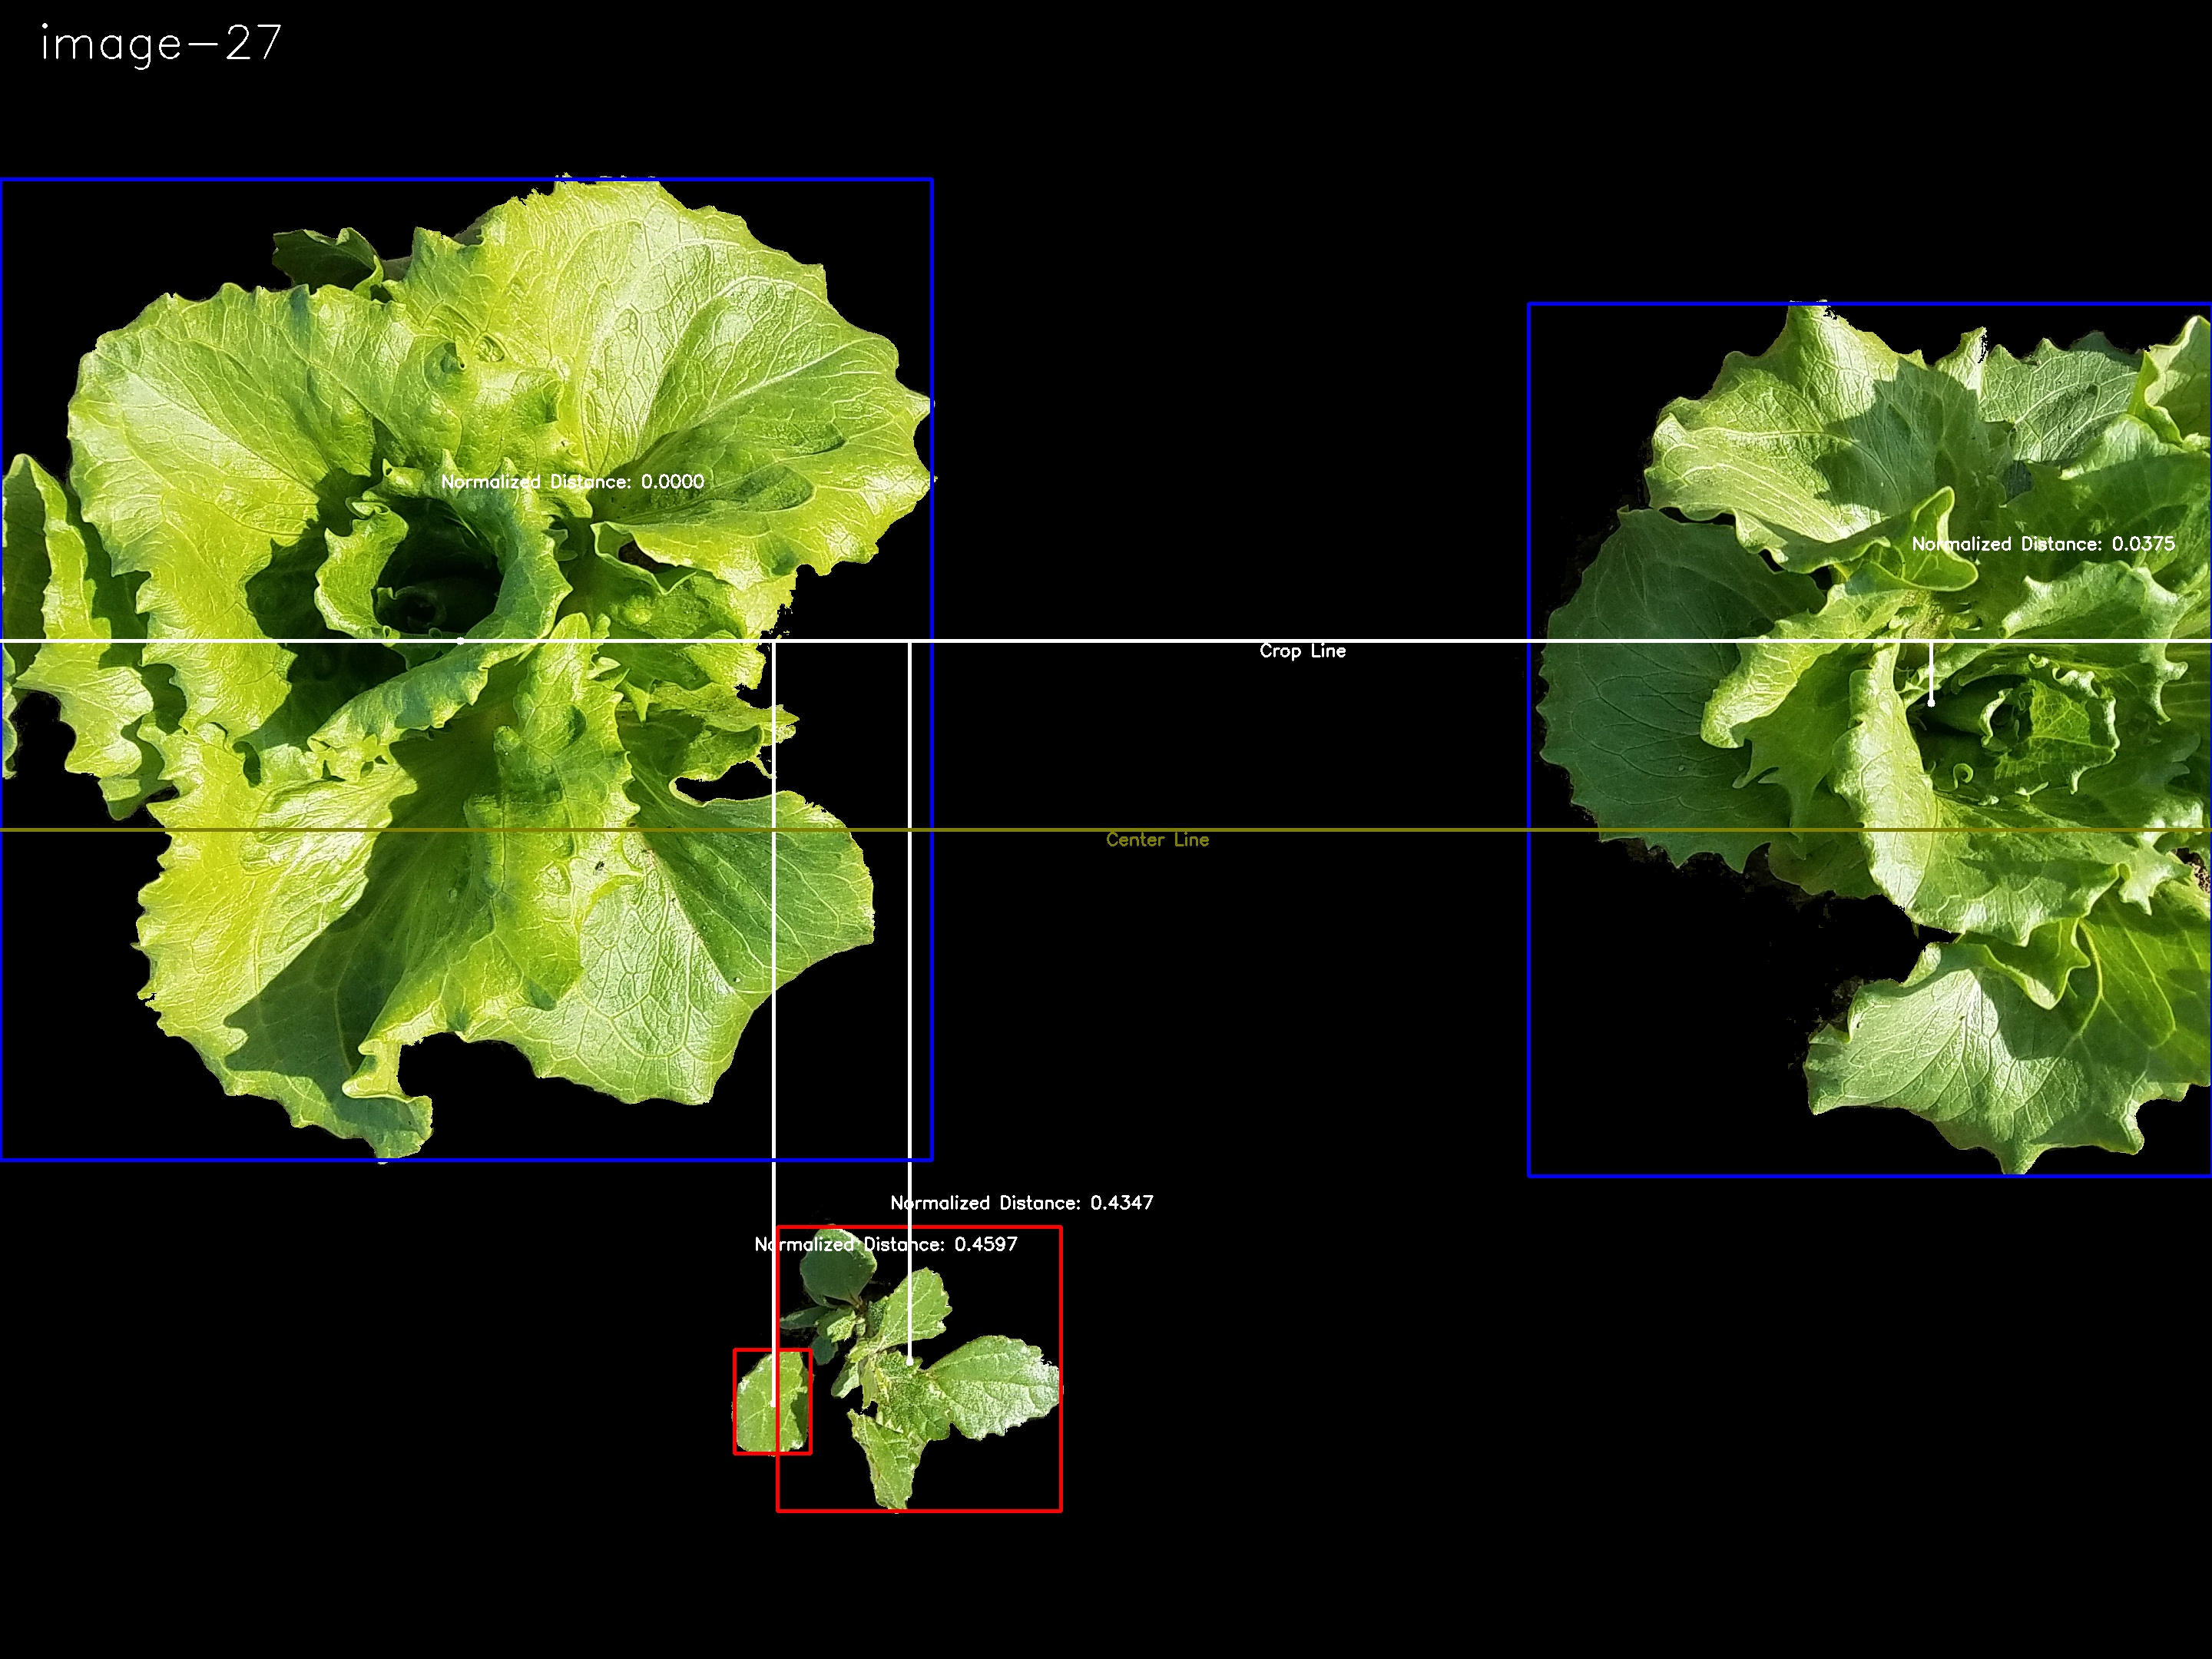
\includegraphics[width=0.4\linewidth]{./figures/normalized-distance.jpg}
	\caption[Distance from Cropline]{Distance from Cropline. Vegetation far from the cropline are most often weeds.}
	\label{fig:normalized-distance}
\end{figure}
Figure~\ref{fig:normalized-distance} illustrates the concept of a cropline and the distance of vegetation from it. In this image we see two growths of lettuce that are very close to the cropline (distances here are in pixels, but the units are not significant. This could be expressed in millimeters) at 0 and 0.375 and a weed lying 0.4347 units from the cropline. The values normalized between 0 and 1 by considering the maximum distance the vegetation could be away from the crop line. The line marked {\it Center Line} is for reference purposes and can be ignored for now.  There are two additional items that are worth noting about this image: the dots connecting the plant to the cropline are the {\it centroids} mentioned earlier, and the colored bounding boxes signify the class of the object, something we will return to in a later section.

\subsection{Histogram of Oriented Gradients}
Often shortened to \textit{HOG}, this technique is a technique to formalize the gradient orientation and magnitude of local portions of an image \parencite[p.~155]{Forsyth2012-hy}. The detail shown in Figure~\ref{fig:hog} is still recognizable as vegetation, but illustrates gradient orientation, not pixel values. It is these orientations that will be exploited in classification, specifically the standard deviation of the gradient descriptors for a plant. In lettuce the orientation of a gradient is visible even to the unaided eye, as the vein structure can be used to classify the image \parencite{Elhariri2014-eo}
\begin{figure}[h!]
	\centering
	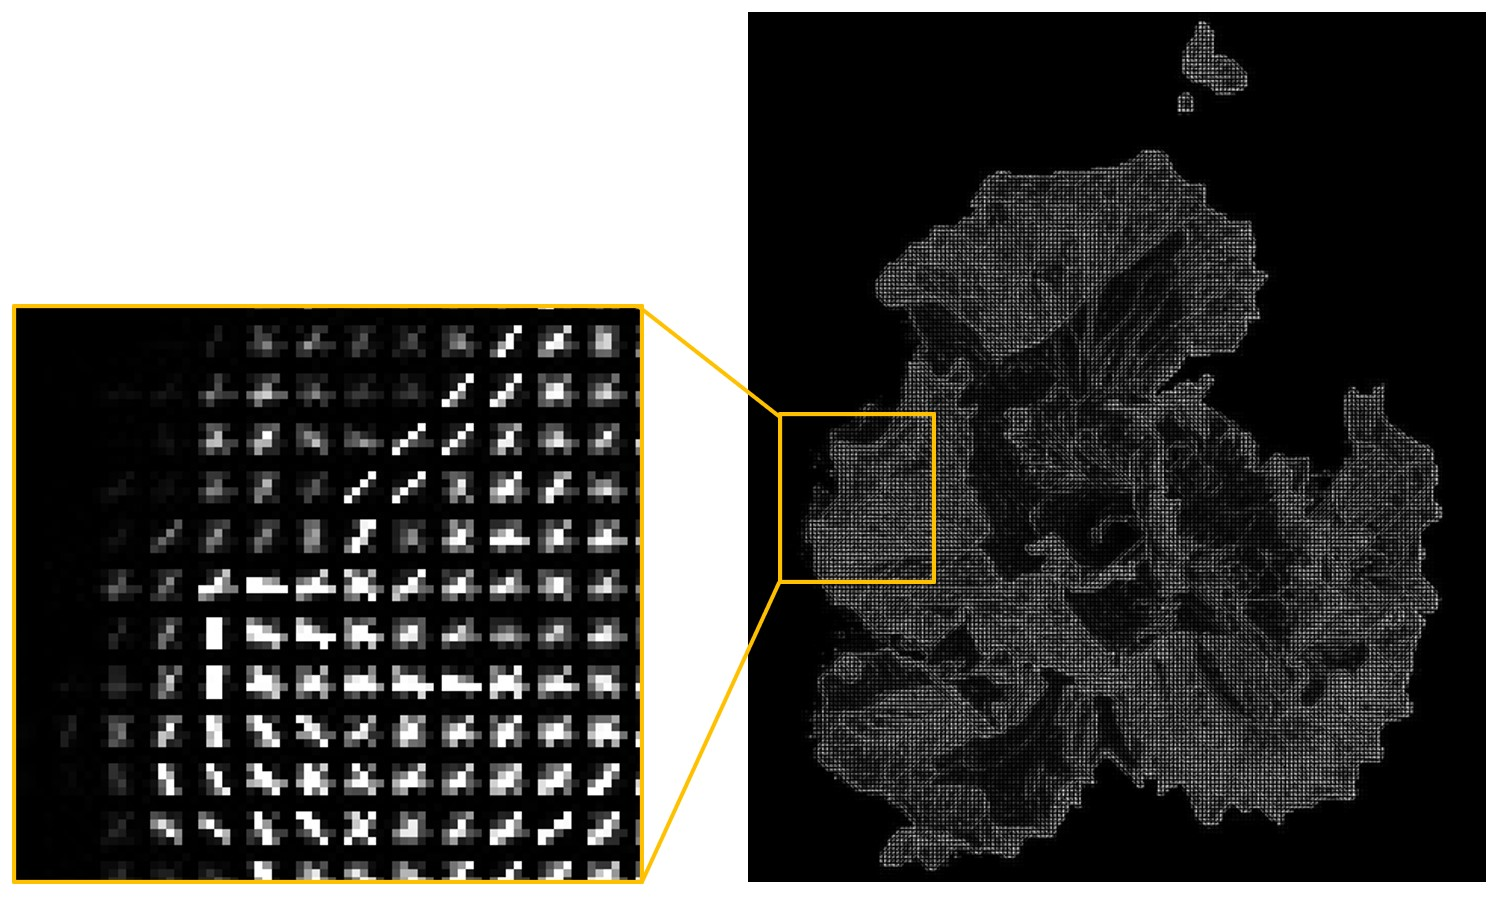
\includegraphics[width=0.4\linewidth]{./figures/hog.jpg}
	\caption[HOG Representation of Lettuce]{HOG Representation of greyscale lettuce image.}
	\label{fig:hog}
\end{figure}

\subsection{Overlapping Vegetation}

Before considering the details of classification, it is worth considering a problem that is sometimes seen: overlapping vegetation. While desired vegetation can overlap itself, this becomes problematic when desired and undesired vegetation overlap. Overlapping vegetation is problematic in the current processing flow in that it is detected as part of the adjoining vegetation, distorting shape analysis computations.  Consider this portion of an image:
\begin{figure}[H]
	\centering
	\begin{subfigure}[h]{.40\textwidth}
		\centering
		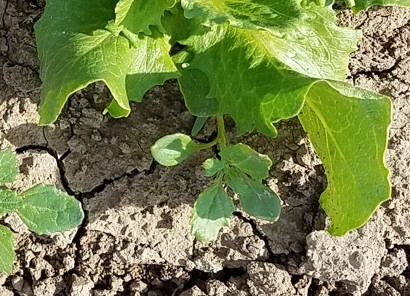
\includegraphics[width=4cm]{./figures/overlapping-weed.jpg}
		\caption{Raw image}
		\label{fig:overlap-raw}
	\end{subfigure}
	\begin{subfigure}[h]{.40\textwidth}
		\centering
		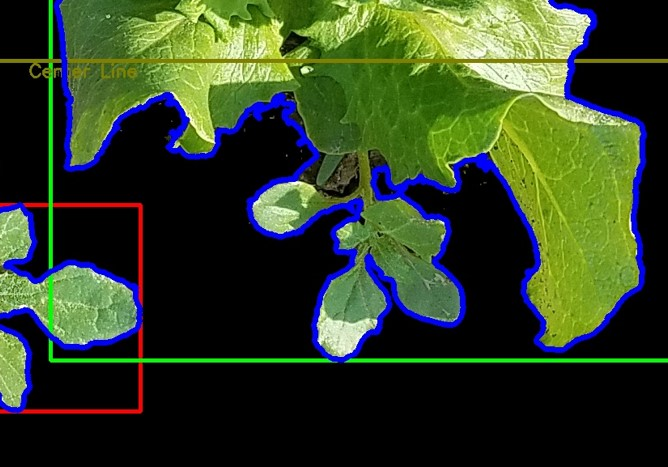
\includegraphics[width=4cm]{./figures/overlapping-weed-segmented.jpg}
		\caption{Segmented image}
		\label{fig:overlap-segmented}
	\end{subfigure}
	\caption[Crop and Weed overlap]{Crop and Weed overlap -- this image contains a problem commonly encountered, the situation where there is overlap between the crop and weeds. In this instance, the crop partially obscures the weed. The blob detection algorithm does not use factors such as color differences to distinguish one blob from another, resulting in two plants being processed as a single one, as can be observed in~\ref{fig:overlap-segmented}}
	\label{fig:overlap}
\end{figure}


The object detection algorithms are based on shapes of binary images, leading to the case where a few leaves of the weed are incorrectly identified as part of the crop. In this case,some leaves are identified as separate plants and are marked as requiring treatment, but this may not be the case with a larger plant requiring treatment that happens to overlap with desired vegetation. This affects not only the inclusion of weeds with crop, but the misidentification of several weeds as a single plant, as this image demonstrates.  Two of the plants in the image are identified as a single blob as the overlapping leaves of multiple plants makes it appear as one. While this a mistake that will result in the distortion of shape metrics, the weed occupies a space so close to the crop that it would not be treated even if properly identified.

\subsection{Weed Shapes and Color}
There are two complications with the identification of weeds by considering shape.  Computation of the shape index of objects within the image are complicated by poor lighting requiring more pixel dilation to make the vegetation appear to be a single plant. This, in turn, distorts the computation of the shape index of the object. The indices covered in Table~\ref{table:segmentation} fail to capture elements of the vegetation that are other than the commonly encountered green.

Consider a sample of Purslane:
\begin{figure}[H]
	\centering
	\begin{subfigure}[h]{.40\textwidth}
		\centering
		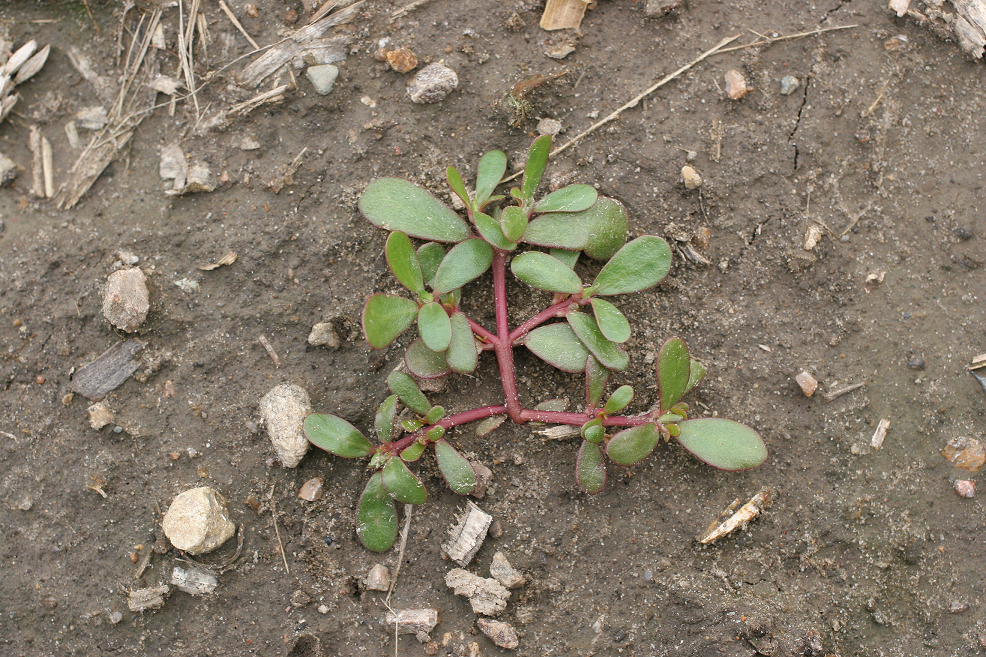
\includegraphics[width=4cm]{./figures/purslane.png}
		\caption{Purslane}
		\label{fig:purslane}
	\end{subfigure}
	\begin{subfigure}[h]{.40\textwidth}
		\centering
		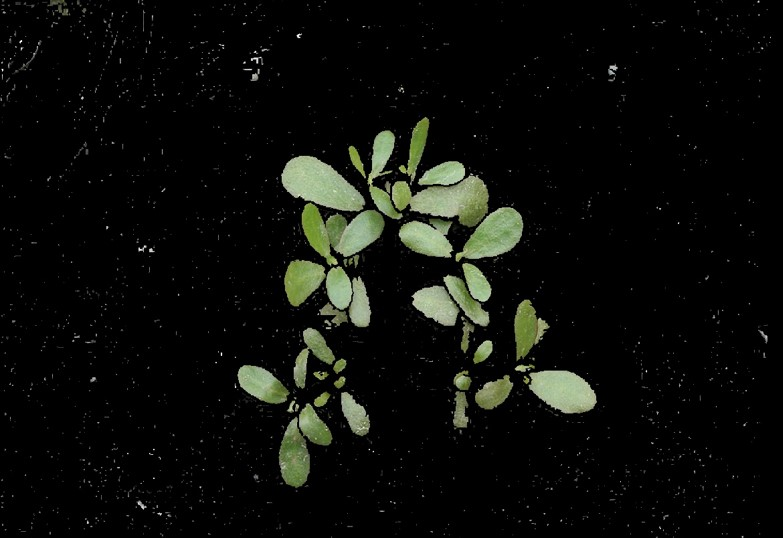
\includegraphics[width=4cm]{./figures/purslane-segmented.jpg}
		\caption{Segmented image (NDI)}
		\label{fig:purslane-segmented}
	\end{subfigure}
	\caption[Color problems complicate segmentation]{The red stems found in purslane complicate use of indices calculated to emphasize green vegetation. As seen in Figure~\ref{fig:purslane-segmented}, the prominent red stems are not present in the final image.}
	\label{fig:purslane-segmentation}
\end{figure}

The color of the purslane stem is a shade of red that is not isolated by considering only a single threshold of the vegetation indices discussed earlier in this document. While using a second threshold value to capture the stems is an option, this approach is complicated by the red content of the background. This problem is not unique to purslane, but can be seen in other vegetation with significant amounts of red in edges of leaves such as found in redroot pigweed (\textit{Amaranthus retroflexus}).  The presence of red in leaves mis-identification of leaves as separate plants (stems) and to the distortion of shape metrics (leaves).



\section{Feature Selection}
The features described in the previous section were generated for a set of segmented images, resulting in each object being described by 715 attributes. Several techniques were then used to explore the relationship between these attributes and the labeled class: Recursive Feature Elimination, Principle Component Analysis (PCA), Feature Importance, and Univariate.  Specifically, only the most important variables will be selected in the predictions, and those parameters with a weak association are dropped. Unfortunately, different feature ranking techniques identified sets of the most significant features without a clear overlap. There were exceptions to this, of course, as can be seen with the feature \textit{saturation\_mean} identified with the highest rank in most of the analysis.
While the features shown in Table~\ref{table:parameters} are not completely consistent with each other there are a few themes:
\begin{itemize}
\item{Aspects of color data are quite predictive, particularly the saturation of the color.}
\item{Most structural attributes (convexity, roundness, etc) are not significant.}
\item{Statistical analysis of the gradients and pixels relationship to each other is significant.}
\end{itemize}


\begin{longtable}{lllll}
\caption[Parameters Identified by Selection Technique]{Parameters Identified by Selection Technique}\\
\toprule
{}Rank &                  Recursive &                       PCA &              Importance &       Univariate \\
\midrule
\endfirsthead
\caption[Parameter Selection by Technique]{Parameter Selection by Technique} \\
\toprule
{}Rank &                  Recursive &                       PCA &              Importance &       Univariate \\
\midrule
\endhead
\midrule
\multicolumn{5}{r}{{Continued on next page}} \\
\midrule
\endfoot

\bottomrule
\endlastfoot
0 &            saturation\_mean &                       hue &     ycbcr-cr\_energy\_avg &  saturation\_mean \\
1 &                 hog\_stddev &           saturation\_mean &   hsi\_saturation\_ASM\_45 &       hog\_stddev \\
2 &               hog\_variance &                  in\_phase &       yiq\_i\_contrast\_45 &         hog\_mean \\
3 &   greyscale\_correlation\_90 &                   cb\_mean &   ycbcr-cb\_contrast\_180 &         in\_phase \\
4 &                   hog\_mean &                hog\_stddev &             cie\_b\_ASM\_0 &     hog\_variance \\
5 &  greyscale\_correlation\_avg &                  hog\_mean &      cie\_a\_contrast\_135 &  ycbcr-cr\_ASM\_90 \\
6 &               yiq\_i\_ASM\_90 &              hog\_variance &      red\_homogeneity\_90 &     value\_ASM\_90 \\
7 &     greyscale\_contrast\_avg &   greyscale\_homogeneity\_0 &     red\_homogeneity\_135 &    value\_ASM\_135 \\
8 &  greyscale\_correlation\_180 &  greyscale\_homogeneity\_45 &  hsv\_saturation\_ASM\_180 &     value\_ASM\_45 \\
9 &    greyscale\_correlation\_0 &  greyscale\_homogeneity\_90 &             red\_ASM\_135 &    value\_ASM\_avg 
\label{table:parameters}
\end{longtable}

The set of unique parameters across the top 10 selection techniques was relatively small, yielding a search space of 348,330,136 combinations. This parameter space was exhaustively searched to find the set of parameters best suited for each of the  seven clasification techniques:
\begin{itemize}
	\item{Random Forest}
	\item{K Nearest Neighbors (KNN)} - The number of neighbors was set to a small value of five.
	\item{Gradient Boosting}
	\item{Logistic Regression}
	\item{Decision Tree}
	\item{Support Vector Machine (SVM)}
	\item{Linear Discriminate Analysis (LDA)}
\end{itemize}

 Table~\ref{table:optimal} contains the result of this search with the accuracy scores using an average across 5 folds.

\begin{tiny}
% -- begin copied table
\begin{longtable}{lllllll}
\caption[Optimal Parameters for Accuracy]{Optimal Parameters by Technique (Accuracy)}
\label{table:optimal-accuracy}\\
\toprule
            RandomForest &                      KNN &         GradientBoosting &       LogisticRegression &
     DecisionTree &                      SVM &                      LDA \\
\midrule
\endfirsthead
\caption[]{Optimal Parameters by Technique (Accuracy)} \\
\toprule
            RandomForest &                      KNN &         GradientBoosting &       LogisticRegression &
     DecisionTree &                      SVM &                      LDA \\
\midrule
\endhead
\midrule
\multicolumn{7}{r}{{Continued on next page}} \\
\midrule
\endfoot

\bottomrule
\endlastfoot
                0.948485 &                 0.948485 &                 0.948485 &                 0.948485 &
         0.948485 &                 0.927273 &                 0.890909 \\
                 cb\_mean &                  cb\_mean &                  cb\_mean &                  cb\_mean &
              cb\_mean &                  cb\_mean &                  cb\_mean \\
      cie\_l\_contrast\_180 &       cie\_l\_contrast\_180 &       cie\_l\_contrast\_180 &       cie\_l\_contrast\_1
80 &       cie\_l\_contrast\_180 &       cie\_l\_contrast\_180 &       cie\_l\_contrast\_180 \\
        green\_contrast\_0 &         green\_contrast\_0 &         green\_contrast\_0 &         green\_contrast\_0 &
         green\_contrast\_0 &         green\_contrast\_0 &         green\_contrast\_0 \\
      green\_contrast\_180 &       green\_contrast\_180 &       green\_contrast\_180 &       green\_contrast\_180 &
       green\_contrast\_180 &       green\_contrast\_180 &       green\_contrast\_180 \\
 greyscale\_homogeneity\_0 &  greyscale\_homogeneity\_0 &  greyscale\_homogeneity\_0 &  greyscale\_homogeneity\_0 &
  greyscale\_homogeneity\_0 &  greyscale\_homogeneity\_0 &  greyscale\_homogeneity\_0 \\
greyscale\_homogeneity\_45 & greyscale\_homogeneity\_45 & greyscale\_homogeneity\_45 & greyscale\_homogeneity\_45 &
 greyscale\_homogeneity\_45 & greyscale\_homogeneity\_45 & greyscale\_homogeneity\_45 \\
greyscale\_homogeneity\_90 & greyscale\_homogeneity\_90 & greyscale\_homogeneity\_90 & greyscale\_homogeneity\_90 &
 greyscale\_homogeneity\_90 & greyscale\_homogeneity\_90 & greyscale\_homogeneity\_90 \\
              hog\_stddev &                 hog\_mean &                 hog\_mean &                 hog\_mean &
             hog\_mean &                 hog\_mean &                 hog\_mean \\
          red\_energy\_avg &             hog\_variance &               hog\_stddev &               hog\_stddev &
            hog\_stddev &               hog\_stddev &               hog\_stddev \\
          ycbcr-cb\_ASM\_0 &                      hue &             hog\_variance &                 in\_phase &
         hog\_variance &             hog\_variance &             hog\_variance \\
\end{longtable}




% -- end copied table
\end{tiny}
 
\subsection{Principal Component Analysis}
The Principal Component Analysis (PCA) \parencite{Muller2016-ui} seen in Figure~\ref{fig:pca} shows most of the variance can be explained by only 3 features: \textit{hue}, \textit{saturation\_mean}, and \textit{in\_phase}.
\begin{figure}[h]
	\centering
	\begin{subfigure}[h]{.48\textwidth}
		  \centering
		  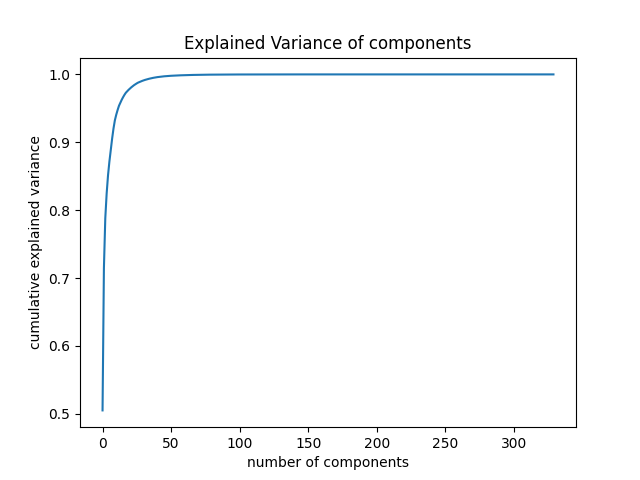
\includegraphics[width=1\linewidth]{figures/pca.png}
		  \caption{Features explaining variance}
		  \label{fig:pca}
	\end{subfigure}
	\begin{subfigure}[h]{.32\textwidth}
	  \centering
	  	
		{
		\centering\settowidth\rotheadsize{\bfseries(our proposal)}
		\renewcommand\theadalign{cl}\renewcommand\cellalign{cl}
		\renewcommand\theadfont{\bfseries}
		\renewcommand\tabcolsep{4pt}\renewcommand\arraystretch{1.25}
		% Make this a bit smaller so it will fit on a page.  Still looks a bit nasty in that it extends to the edge of the page.
		% It's that PCA line that is the trouble, as the values are just too long
		\footnotesize
		
		\begin{longtable}[c]{
		    |l |*{12}{c |} }%
		    \hline
		    %\diagbox[height=1.2\rotheadsize, width=\dimexpr\eqboxwidth{AB}+2\tabcolsep\relax]%
		    %{\raisebox{1.2ex}{Feature}}{\raisebox{-5ex}{Feature}} &
		    {\textbf{Feature}} & {\textbf{Importance Rank}}\\
		    %\rothead{Tool X\\\mbox{(our proposal)}}\\
		    \hline
			hue                      &     0.505089 \\
			saturation\_mean          &     0.209646 \\
			in\_phase                 &     0.073444 \\
			cb\_mean                  &     0.036392 \\
			hog\_stddev               &     0.026874 \\
			hog\_mean                 &     0.020135 \\
			hog\_variance             &     0.017359 \\
			greyscale\_homogeneity\_0  &     0.016602 \\
			greyscale\_homogeneity\_45 &     0.014872 \\
			greyscale\_homogeneity\_90 &     0.012052 \\	    
		    
		    \hline
		    %\caption{Feature Importance Ranks using RFE with a Random Forest Classifier}
		    %\label{fig:random-forest}
		  \end{longtable}
		 }
	  \caption{PCA Variances}
  %\label{fig:sub2}
	\end{subfigure}
\caption{Principal Component Analysis of Features}
\label{fig:pca}
\end{figure}




 
  Given these observations, we can use these parameters for our training and prediction:
 \begin{itemize}
	\item{The length/width ratio}
	\item{The shape index}
	\item{The YIQ in-phase mean}
	\item{The distance from the cropline}
\end{itemize}

Plotting these attributes along with their classification via Logistic Regression yields Figure~\ref{fig:factors}. This plot shows that items correctly classified as weeds are are tightly grouped. Vegetation correctly classified as crop shows a somewhat looser, but still quite evident grouping.
 \begin{figure}[H]
	\centering
	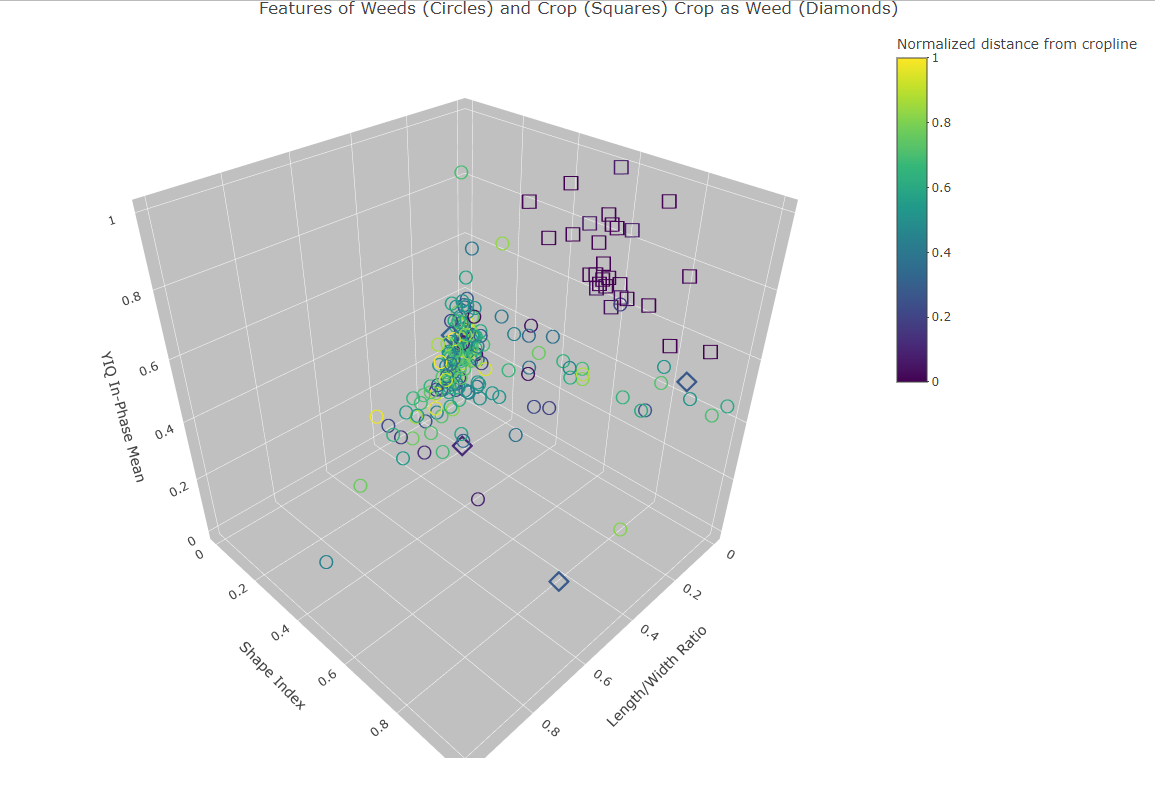
\includegraphics[width=0.9\linewidth]{./figures/plot-factors.png}
	\caption[Factors selected for discrimination]{A plot of the four factors selected with the shape noting the true classification of the blob. In this graph the factors selected occupy space and color, with the shape of the object noting the classification.}
	\label{fig:factors}
\end{figure}
  
\section{Classification}

Using the subset of the parameters identified in the previous section, various approaches were used in classifying the objects isolated in the images and detailed in Table~\ref{fig:learning}. The feature sets were split into a 80\%/20\% for these results: 

{\renewcommand{\arraystretch}{2}%
\begin{table}[H]
	\centering
    \caption{Learning Results}
    \label{fig:learning}
    \begin{tabular}{  l  p{4cm}  p{5cm} }
     %\begin{tabular}{  l  p{3.4cm}  p{3.4cm} }
        \toprule
\textbf{Method}      
& \textbf{Train}   
& \textbf{Test} \\\midrule
Random Forest      
& 1.0
& 0.986 \\\hline
Logistic Regression
& 0.9790       
& 0.9787 \\\hline
Decision Tree
& 1.0
& 0.96 \\\hline
Boosted Gradient     
& 1.0
& 0.957 \\\hline
KNN     
& $1.0$                    
& $0.86$ \\\hline
        \bottomrule
    \end{tabular}
\end{table}

For this sample dataset, all approaches with the exception of KNN yield commercially acceptable results if accuracy were the only criterion used in evaluation. However this case must consider two other criteria that are important, but beyond the scope of this document:
\begin{itemize}
\item{The computational cost of achieving each result. The prediction will be done in real-time under field conditions\footnote{And on a GPU, not on a CPU as was done here} While a result of an approach yielding results above 98\% may sound impressive, if that prediction using logistic regression takes a few hundred milliseconds and a decision tree takes well under 100 milliseconds, it may be the case that using that logistic regression in practice is not viable.\footnote{Some context is probably needed here. This prediction will be done as a tractor is moving along, and the time spent on prediction is part of an overall time budget that will ultimately limit the forward speed of the tractor. 2 MPH is commercially viable. 1 MPH is not.}}
\item{The cost of misclassifying a crop as a weed has very real dollar cost, as the subsequent killing of that plant would negatively impact the total crop suitable for sale. The cost of classifying a weed as a crop (and thus not flagging it for treatment) is much lower. While it may have modest financial impact, as leaving the weed in place allows it to take resources away from marketable vegetation (water, fertilizer), the impact of doing so may be acceptable in most instances.}
\end{itemize}
 
Misclassification rates where crop is identified as a weed is the most pressing concern here, so it is worthwhile evaluating the performance of these approaches with the goal of minimizing that class of misclassification while maximizing the correct classification of weeds as weeds. Figure~\ref{fig:classification-rates} addresses this goal by showing percentages of correct and incorrect classifications. While there several approaches showed quite similar acceptable  results (SVM, Random Forest, and Logistic Regression) and three approaches with unacceptable results (KNN, Boosted Gradient, and Decision Tree). While it is likely the case that the unacceptable approaches can be optimized to the point that their results would migrate them to the acceptable category, this paper will concentrate only on the approaches will acceptable results.

\begin{figure}[h]
	\centering
	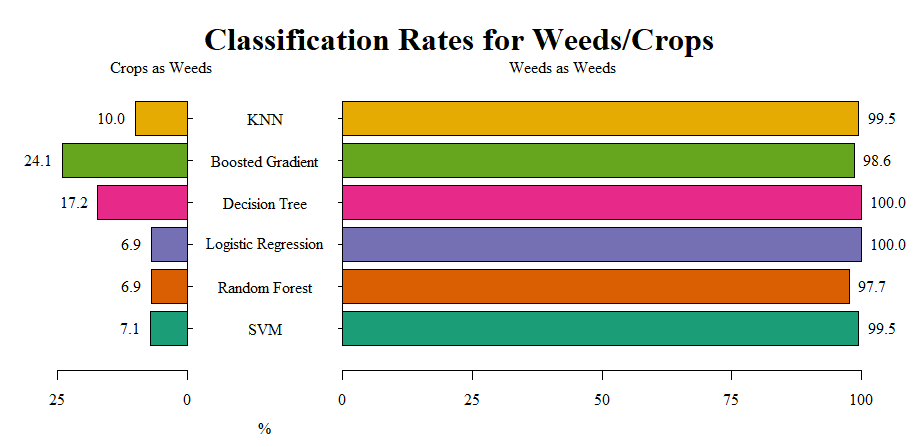
\includegraphics[width=0.7\linewidth]{./figures/classification-rates.png}
	\caption[Misclassification rates of various algorithms]{The correct and misclassification rates of various algorithms are shown here. While an overall accuracy of 95.7\% may sound impressive for the Boosted Gradient algorithm (See Table~\ref{fig:learning}), considering the salient misclassification and correct classification rates, 24.1\% and 98.6\%, respectively, that algorithm does not support the accuracy needed in this use case.}
	\label{fig:classification-rates}
\end{figure}

Figure~\ref{fig:classified} shows an annotated classification result. In this figure, we see desirable (crop) bounded by a green box, and undesirable (not crop) bounded in red. The blue box bounds vegetation for which we can't reliably determine its class. Computations that depend on an unimpeded view of the vegetation ({\it length/width ratio}, for instance) can't be reliably performed, so classification of elements that are not fully captured are not classified. Some color computations could be, but may not be as representative as required. The {\it hue} value, for example, is the mean value across the entire plant, and the hue may not be consistent across the entire plant. The portion that is visible may not be representative of the plant as a whole.

\begin{figure}[H]
	\centering
	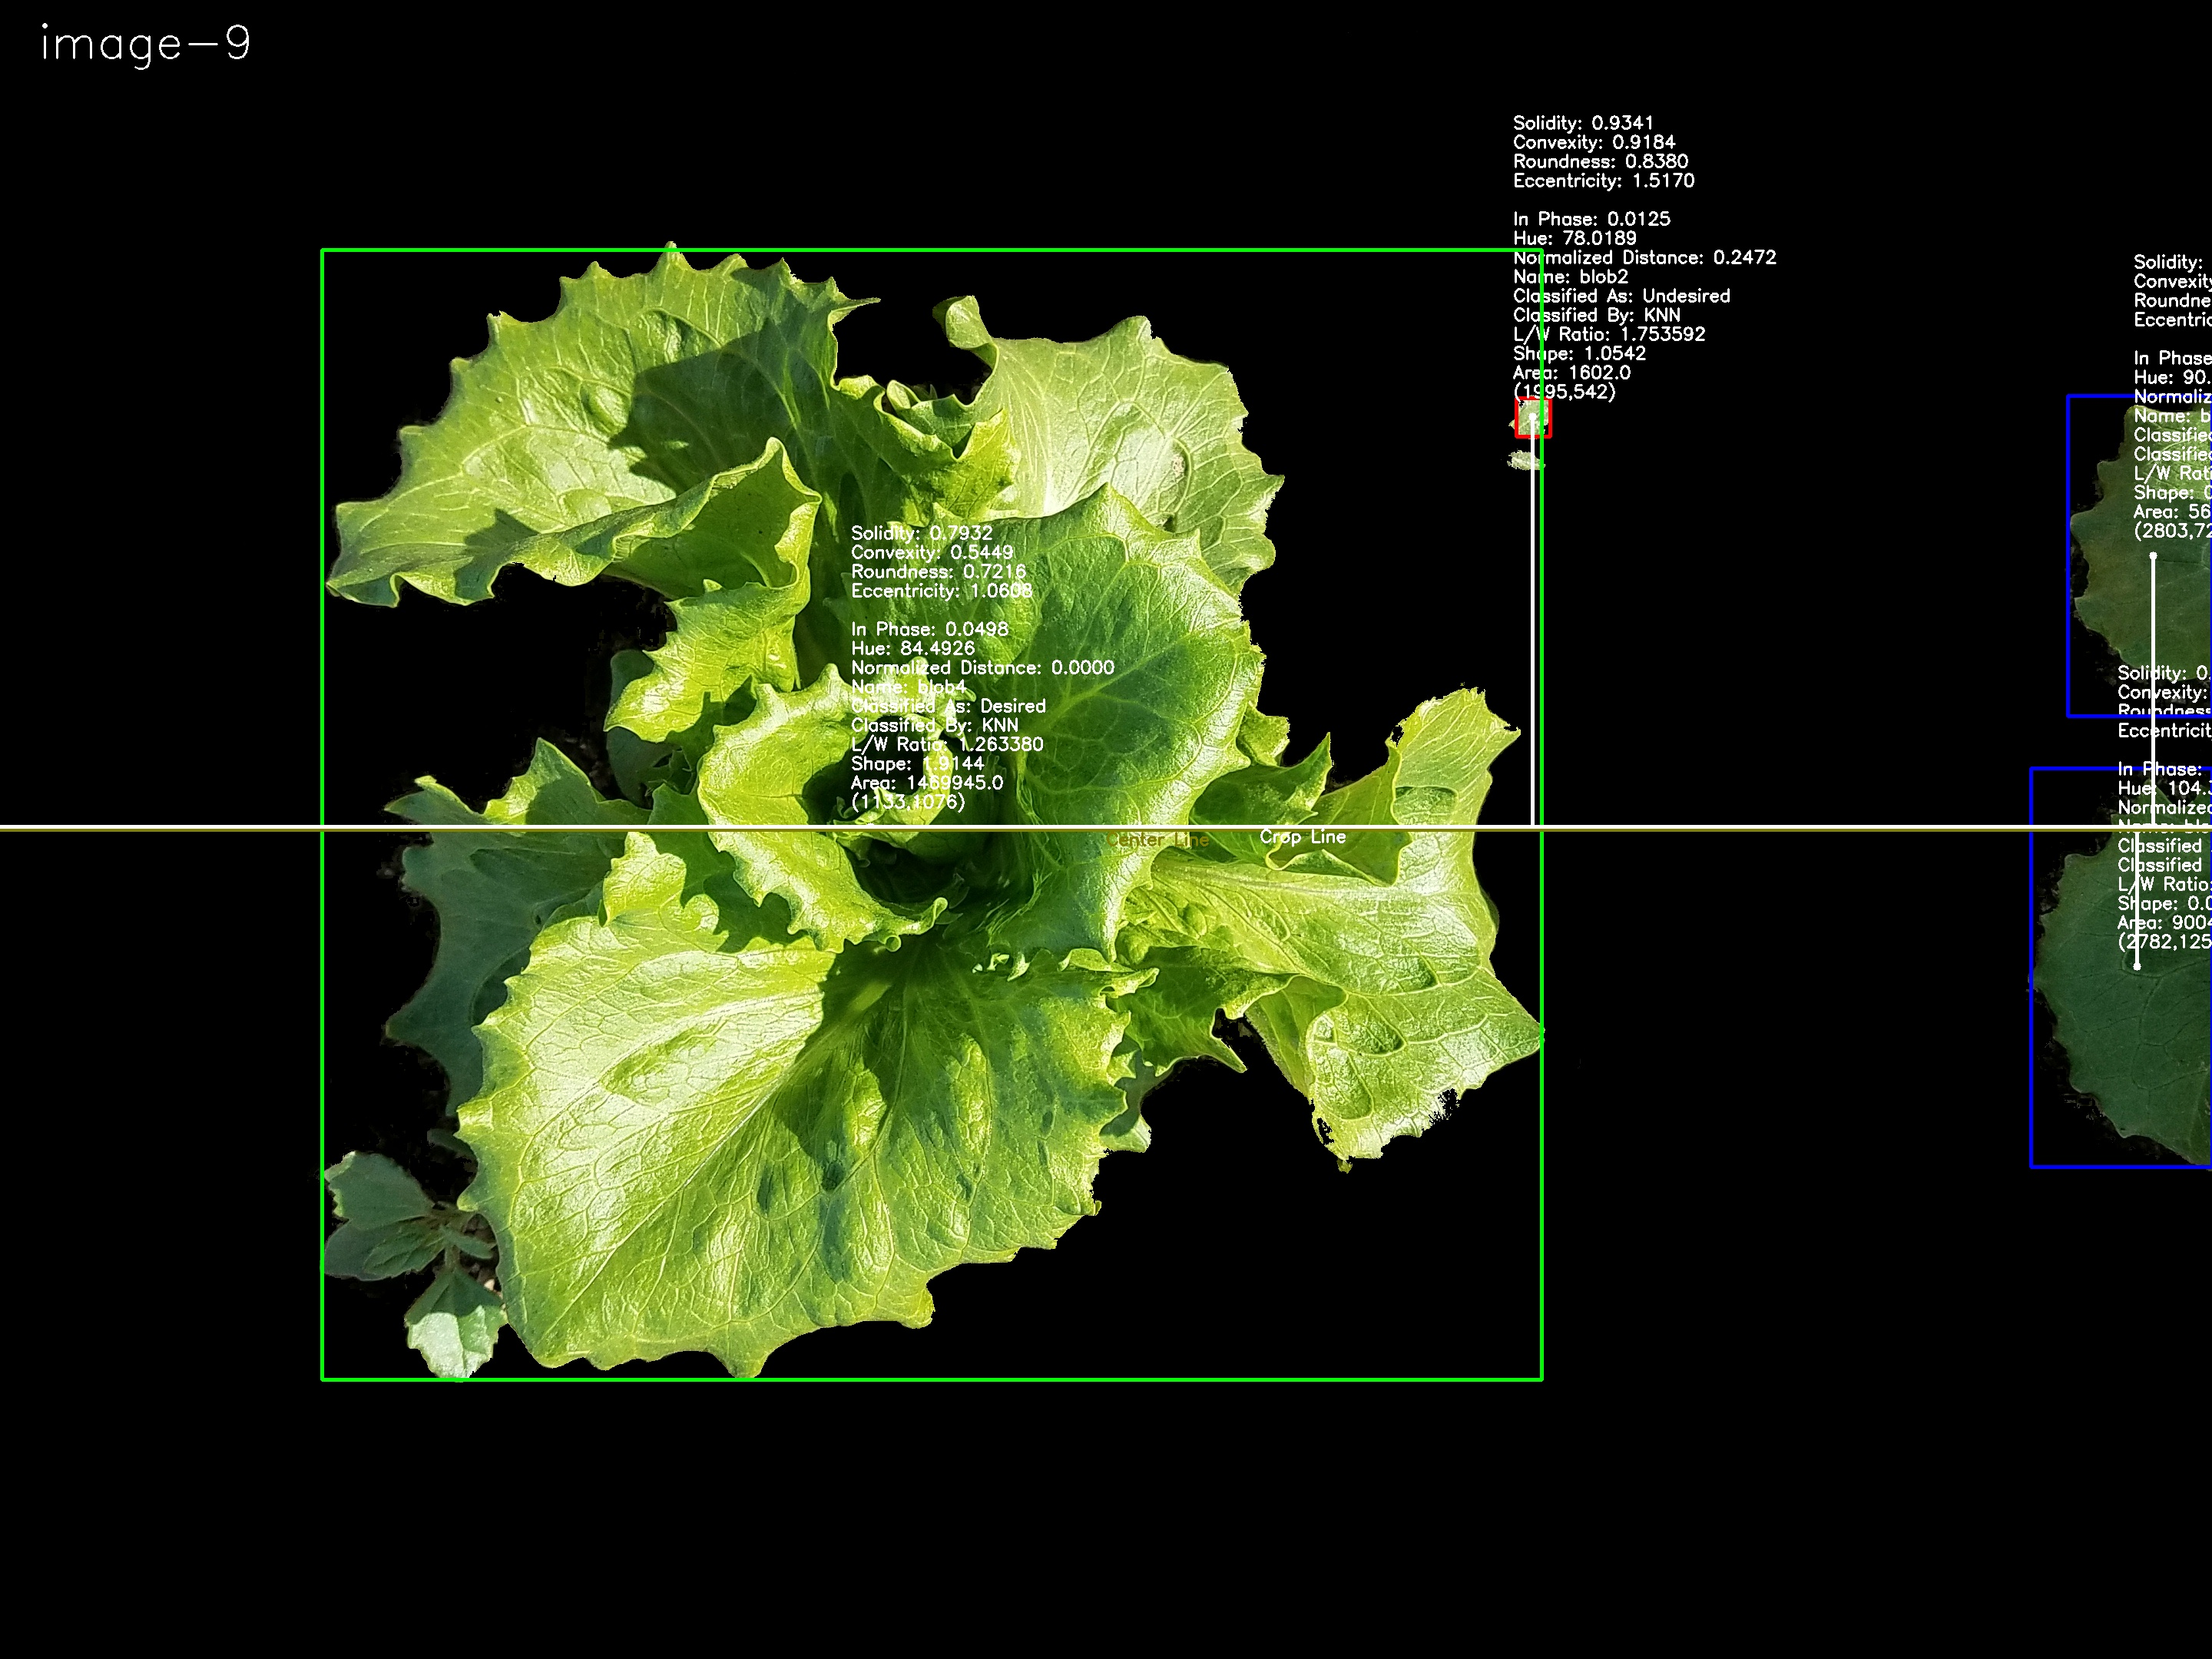
\includegraphics[width=0.7\linewidth]{./figures/classified-result.jpg}
	\caption[A classified and annotated image]{A classified result. Desirable vegetation is bounded in green and undesirable in red. Note that this image also demonstrates a commonly encountered problem, that of overlapping vegetation. In the lower left of the green bounding box there is a weed that is overlapped by crop vegetation. In this case, however, the weed's proximity to the crop makes treatment problematic in that doing so represents a risk of producing crop damage.}
	\label{fig:classified}
\end{figure}

\newpage
\section{References}
\printbibliography[heading=none]

%\cite{Wirth2004-li}
\end{document}

